\documentclass[UTF8,nofonts,cs4size]{ctexrep}
\setCJKmainfont{AR PL SungtiL GB} %中文为wqy 微米黑字体
\usepackage{amsmath, amsfonts}
\usepackage{graphicx}
%插入c代码
\usepackage{xcolor}
\usepackage{listings}
\lstset{
  language=C,
  keywordstyle=\color{blue},
  numbers=left,
  basicstyle=\ttfamily,
  frame=leftline,
  breaklines=true,
  texcl=true,
%  backgroundcolor=\color{green!69!yellow!30!}
}


\usepackage[top=3.8cm,bottom=3.8cm,left=3.8cm,right=2.8cm]{ geometry}
\usepackage{indentfirst}
\setlength{\parindent}{2em }
\setlength{\parskip}{0pt }

%页眉和页脚
\usepackage{fancyhdr}
\pagestyle{fancy}
\lhead{}
\chead{\zihao{-5} 青岛理工大学毕业论文(设计)}
\rhead{}
\lfoot{}
\cfoot{\thepage}
\rfoot{}

\begin{document}
%章节格式设置
\CTEXsetup[format={\centering\zihao{3}}]{chapter}
\CTEXsetup[format={\bf\zihao{4}}]{section}
\CTEXsetup[format={\bf\zihao{-4}}]{subsection}
%章节前后


\CTEXsetup[beforeskip=18pt]{chapter}
\CTEXsetup[afterskip=24pt]{chapter}
%节前后
\CTEXsetup[beforeskip=6pt]{section}
\CTEXsetup[afterskip=24pt]{section}
%分节前后
\CTEXsetup[beforeskip=6pt]{subsection}
\CTEXsetup[afterskip=12pt]{subsection}
%目录格式设置
\CTEXoptions[contentsname={\zihao{3}目\ 录}]
\tableofcontents
%段前段后距离设置
\CTEXsetup[beforeskip=0ex]{paragraph}
%\CTEXsetup[afterskip=0ex]{paragraph}
%摘要
\CTEXoptions[abstractname={\zihao{3}摘\ 要}]
\begin{abstract}
\indent \ \ \ \ \ 
操作系统是计算机体系中最为重要的系统软件,是架构在硬件之上的资源管理者,也是用户和硬件之间的桥梁。而在当下的计算机操作系统教学过程中,主要以理论为主,缺少学生自己动手实现的环节。本设计针对IA32架构的硬件系统,使用Nasm和C
语言作为开发工具,使用Make自动编译工具构建编译环境,使用bochs和gbd作为调试开发工具,系统架构在Ubuntu10.10之上,设计并且实现了一个实时多进程操作系统。系统启动过程分成了三个步骤:加载boot、加载loader、加载内核。该系统实现了操作系统的基本功能:内存管理,进程管理,一个简单的文件系统和其他一些辅助功能。系统采用微内核结构,系统中各个进程之间通过一个同步IPC的机制交互信息。内存在基本的段页式管理机制基础上,开辟出10MB以上的空间作为用户空间,并实现了一种简单的分配机制。该操作系统实现了一套完整的进程管理机制,包括:PCB,进程初始化,进程调度 、中断服务系统、时钟中断等服务。各进程之间共享CPU,通过进程调度机制来获得CPU使用权并运行。并通过系统调用的形式向编程人员提供了各种接口。并且实现了一个简单的shell,用户可以在该操作系统上运行自己的程序。

\paragraph{}
\noindent{\bf\zihao{-4}[关键词:]}操作系统;IA32;进程管理;内存管理
\end{abstract}


%摘要
\CTEXoptions[abstractname={\zihao{3}ABSTRACT}]
\begin{abstract}
\indent \ \ 
Operating system is the most important computer system software, is the architecture of hardware on the resource managers, but also a bridge between the user and the hardware. The computer operating system in the present process of teaching, mainly in theory, the lack of links students to achieve their own hands. So we focused on IA32 hardware system architecture, design and implementation of a real-time multi-process operating system. System startup process into three steps: load boot, load the loader, load the kernel. The system implements the basic functions of the operating system: memory management, process management, a simple file system and other auxiliary functions. System uses a micro-kernel structure, system, each process synchronization between the IPC by a mutual information mechanism. Section of the memory page in the basic style management, based on more than 10MB of space opened up as a user space, and to achieve a simple distribution mechanism. The operating system implements a complete set of process management mechanisms, including: PCB, process initialization, process scheduling, interrupt service system, the clock interrupt services. Shared between the processes CPU, through the process of scheduling to get the CPU right to use and run. Form through the system call to provide a variety of programming interfaces. And implements a simple shell, users can run the operating system with their own procedures. 

\paragraph{}
\noindent{\bf\zihao{-4}[Keywords:]}OS;IA3;Process Management;Memery Management 
\end{abstract}



\pagenumbering{arabic}
\chapter{前言}
\section{概述}
操作系统(Operating System)是计算机体系里面最为基础和重要的系统软件。它是用户与计算机硬件系统之间的接口,也是系统资源的管理者,更是用户使用的平台。真正意义上的操作系统主要有四个特点:用户依靠操作系统方便的使用计算机即软件、硬件设备,提高计算机的效率。操作系统必须具有良好的扩充性、优良的移植性、互操作性和统一的开放环境。操作系统是一个非常复杂的知识体系,它涉及的知识很多很复杂,比如内核的研究、进程管理、存储器管理、文件管理和设备管理等技术。目前对于操作系统教材上只讲其原理,不实际动手操作及实现,所以学生在学习它的时候会感到非常抽象。在国内外一些著名高校通常是鼓励学生在学习这门课程的同时自己动手开发一个能够实现OS基本功能的微型操作系统来加强对该课程的掌握。通过实践对于学生充分掌握书本知识、打下扎实的基本功有非常大的帮助。同时,国内操作系统的研发和生产相对于国外来说还相对落后。在操作系统市场上主流的还是微软的Windows系列还有GNU项目的各种Linux发行版本。很少见到国人自主研发的操作系统。即使最近比较流行的麒麟操作系统和雨林木风操作系统也是在GNU项目基础上进行的二次开发,自主研发操作系统的关键技术还是较少。于是本设计想通过自己设计并实现一个操作系统,了解并阐释一个操作系统是如何架构起来的。并对实现一个操作系统的关键技术进行一次实践,为以后开发自己的操作系统做个铺垫。
\section{操作系统的功能}
本设计可以从不同的角度来观察操作系统在整个计算机体系结构中所起到的作用。假若从一般用户的角度看来,可以把操作系统堪称是用户与计算机硬件字同之间的接口;从资源管理的角度看来,操作系统是计算机资源的管理者。
\subsection{操作系统作为用户与计算机之间的接口}
操作系统作为用户与计算机硬件系统之间接口的含义是:操作系统处于用户与计算机硬件系统之间,用户通过操作系统来使用计算机系统。或者说,用户在操作系统的帮助下,能够方便、快捷、安全、可靠的操作计算机硬件和运行自己的程序。应注意,OS是一个系统软件,因而这种接口是软件接口。而本设计所设计的操作系统,面向一般用户的接口为字符中终端,用户通过一个简单的shell来控制系统完成功能。同时面向程序设计人员,开放了系统的编程接口。
\subsection{操作系统作为计算机系统资源的管理者}
在一个计算机系统中,通常都含有各种各样的硬件和软件资源,归纳起来可将资源分为四类:处理器、存储器、I/O设备以及信息。相应的,操作系统的主要功能也是针对这四类资源进行有效的管理,即:处理机管理,用于分配和控制处理机;存储器管理,主要负责内存的分配与回收;I/O设备管理,负责I/O设备的分配和操纵;文件管理,负责文件的存取、共享和保护。可见,操作系统是计算机系统资源的管理者。事实上,当今世界上流行的一个关于操作系统作用的观点,正式吧操作系统作为计算机系统的资源管理者。
\subsection{操作系统用作扩充机器}
对于一台请按全没有软件的计算机(即裸机),即是其功能再强,也必定是难于使用的。如果本设计在裸机上覆盖上一层I/O设备管理软件,用户就可以利用它所提供的I/O命令,来进行数据输入和打印输出。此时用户所看到的机器,将是一台比逻辑功能更强、使用更加方便的机器。通常本设计把覆盖了软件的机器称作是扩充机器或虚机器。如果本设计又在第一层软件之上再覆盖一层管理软件,则用户就可以利用该软件提供的文件存取命令,来进行文件的存取。此时,用户所看到的是一台功能更强的虚机器。由此可知,当本设计在计算机系统上覆盖上一层软件后,系统功能便增强一级。由于操作系统自身包含了很多层次,因此当在裸机上覆盖上操作系统后,便可获得一台宏能增强、使用极为方便的多层扩充机器或者多层虚机器。
\section{定位:实时操作系统}
实时操作系统是指当外界事件或数据产生时,能够接受并以足够快的速度予以处理,其处理的结果又能在规定的时间之内来控制生产过程或对处理系统作出快速响应,并控制所有实时任务协调一致运行的操作系统。因而,提供及时响应和高可靠性是其主要特点。实时操作系统有硬实时和软实时之分,硬实时要求在规定的时间内必须完成操作,这是在操作系统设计时保证的;软实时则只要按照任务的优先级,尽可能快地完成操作即可。虽然本设计设计的操作系统的主要目的在于教学上的应用,但是作为一个实时操作系统只要稍加改造就可应用于一些对实时性要求比较高的场合,比如生产线的控制和机器人控制。
\subsection{所设计实时操作系统特征}
\subsubsection{高精度的计时系统}
计时精度是影响实时性的一个重要因素。在实时应用系统中,经常需要精确确定实时地操作某个设备或执行某个任务,或精确的计算一个时间函数。这些不仅依赖于一些硬件提供的时钟精度,也依赖于实时操作系统实现的高精度计时功能。
\subsubsection{多级中断机制}
一个实时应用系统通常需要处理多种外部信息或事件,但处理的紧迫程度有轻重缓急之分。有的必须立即作出反应,有的则可以延后处理。因此,需要建立多级中断嵌套处理机制,以确保对紧迫程度较高的实时事件进行及时响应和处理。而在本设计所设计的操作系统中,本设计实现了一个多级终端机制。允许终端嵌套。
\subsubsection{实时调度机制}
实时操作系统不仅要及时响应实时事件中断,同时也要及时调度运行实时任务。但是,处理机调度并不能随心所欲的进行,因为涉及到两个进程之间的切换,只能在确保“安全切换”的时间点上进行,本设计在系统中建立更多“安全切换”时间点,保证及时调度实时任务。
\section{进程管理}
进程是操作系统中最为重要的一个观念。                                                                                                                                                                                                                                                                                                                                                                                                                                                                                                                                                                                                                                                                                                                                                                                                                                                                                 从功能上看他是程序的一次执行过程。是伴随着操作系统而诞生的一个概念,也就是说有了操作系统,就有了进程。但是那时本设计并没有给这个执行过程一个抽象的概念。在古老的操作系统中,进程是顺序执行的。只有当一个进程执行完成后,才会让出CPU使用权让下一个进程执行。但是在有了中断管理和多道程序的概念之后,操作系统允许一个正在执行的程序被打断,让CPU转去运行另外的程序。也允许多个程序并发执行。这个时候程序在运行过程中具有了间断性、不封闭性、不可再现性。单纯的顺序调度已经不能够满足要求。于是引入了进程的概念,这也是为了使程序能够并发执行,并且为了对并发执行的程序加以控制和描述。进程是一个动态的使用系统资源、处于活动状态的程序。他记录着一个正在运行的程序的关键信息,也是操作系统对其进行调度的依据。纵观当下主流的操作系统微软的Windows系列、以Linux内核为核心的各种Linux发行版、BSD和Unix等等,都有进程的念。当然这些操作系统是通用操作系统,可以适用于多种环境下。而本设计所设计的操作系统则相对比较简单,只是实现了一个操作系统的框架。但这个操作系统也是一个多任务操作系统,在同一个时间段内允许多个进程并发执行。并且操作系统使用合适的调用算法来调用这些进程。操作系统定为为实时操作系统。在这样一个操作系统中,进程更是起到了举足轻重的作用。进程管理由进程控制块(PCB)、进程调度、中断处理、定时器、进程通信等部分组成,他是本设计所设计的操作系统存储管理、文件管理等其他功能的基础。
\section{实现环境介绍}
在实现本设计所设计的操作系统的时候。本设计主要使用了nasm语言和c语言。其中使用nasm汇编语言完成大部分与硬件交互的代码,而使用c语言完成了一些比较靠上的服务,例如文件系统。并且在linux环境下使用bochs搭建了实验平台,方便测试和调试。
\subsection{开发工具}
\subsubsection{Bochs}
Bochs是一种十分轻便的使用c++编写的开源IA-32(x86)电脑模拟器,可以运行在最受欢迎的平台上。它仿真英特尔x86 CPU、常见的I/O设备、和定制的BIOS。目前,Bochs可以被编译仿真386、486、Pentium/PentiumII/PentiumIII/Pentium4或x86-64位的CPU,包括可选的MMX,SSEx和3DNow指令。在Bochs仿真环境里能够运行许多操作系统,比如Linux、DOS、Windows 95/98/NT/2000/XP或者Windows Vista。Bochs是由凯文·劳顿编写的,目前由“http://bochs.sourceforge.net”的Bochs项目组维护。Bochs可以被编译运用在多种模式下,其中有些仍处于发展中。bochs的典型应用是提供x86 PC的完整仿真,包括x86处理器、硬件设备、和存储器。这让您在您的工作站上的模拟器里运行操作系统和软件,就像你有一台机器内的机器。例如,Bochs还将允许您在安装X11的Solaris机上运行windows应用程序。Bochs的发布遵守GNU LGPL。
\subsubsection{Nasm}
NASM 是一个为可移植性与模块化而设计的一个 80x86 的汇编器。它支持相当多的目标文件格式,包括Linux和'NetBSD/FreeBSD','a.out','ELF','COFF',微软16位的'OBJ'和'Win32'。它还可以输出纯二进制文件。它的语法设计得相当的简洁易懂,和Intel语法相似但更简单。它支持'Pentium','P6'指令集。
\subsubsection{Gcc}
Linux系统下的gcc(GNU C Compiler)是GNU推出的功能强大、性能优越的多平台C语言编译器,是GNU的代表作品之一。gcc是可以在多种硬体平台上编译出可执行程序的超级编译器,其执行效率与一般的编译器相比平均效率要高20%~30%。
\subsection{开发环境}
\subsubsection{Linux}
Linux,是一类Unix计算机作业系统的统称。该作业系统的核心的名字也是“Linux”。Linux作业系统也是自由软体和开放原始码发展中最著名的例子。严格来讲,Linux这个词本身只表示Linux核心,但在实际上人们已经习惯了用Linux来形容整个基于Linux核心,并且使用GNU工程各种工具和资料库的作业系统(也被称为GNU/Linux )。基于这些组件的Linux软件被称为Linux发行版。一般来讲,一个Linux发行套件包含大量的软件,比如软件开发工具、资料库(例如 PostgreSQL、MySQL)、网路伺服器(例如Apache)、X Window 、桌面环境(例如GNOME和KDE)、办公套件(例如OpenOffice.org)、脚本语言(例如Perl、PHP和Python)等等。Linux核心最初是为英特尔386微处理器设计的。现在Linux核心支援从个人电脑到大型主机甚至包括嵌入式系统在内的各种硬件设备。现在,Linux已经成为了一种受到广泛关注和支持的作业系统。包括国际商用机器公司和惠普 、戴尔在内的一些资讯业巨头也陆续支援Linux,并且成立了一些组织支持其发展,如 Open Invention Network(OIN)(成员有IBM、索尼 、NEC、Philips、Novell和Red Hat等)购买了微软专利,允许任何个体以开放的原则使用。很多人认为,和微软的Windows相比,作为自由软件的Linux具有低软体成本、高安全性且可更加信赖等优势,但是同时却需要更多的人力成本。

\chapter{操作系统的结构设计}
\section{设计概要}
操作系统在整个计算机体系结构中占到了非常重要的地位。是硬件系统之上为其他功能提供支柱性作用的系统软件。而设计一个操作系统,其要提供的功能对于硬件而言来说具有极强的针对性。因为在设计操作系统之前,需要明确操作系统所支持的硬件结构。并且还要明确所要设计的操作系统所能够提供的服务。而本设计所设计的这个操作系统,带有极强的实验性质。是对于特定硬件的操作系统。本设计所设计的操作系统针对以Intel80386中央处理器为核心的IA32架构的机器,并且提供了以下功能:文件系统,进程管理,内存管理,进程间通信,基本输入输出系统。并且本设计将这个操作系统定位为教学用实时操作系统。而本文着重研究了操作系统中最为关键的技术——进程管理。从如何控制进程、进程间调度、进程的创建和撤销等角度,探讨了进程管理的一些技术实现。
\section{硬件模型}
硬件是用户最先看到的计算机系统的物理部分,也是操作系统的基石。硬件系统确定了该计算机系统所支持的指令系统,以及程序的运行环境,是一个计算机系统最为关键的部分。本设计在设计操作系统时,必然应当先确定硬件模型。作为系统软件的设计者,本设计所关心并非是硬件的所有的细节,而是对于作为系统程序编程人员的本设计而言,不是透明的那部分。图\ref{hard}展示了本设计所设计的操作系统所针对的硬件模型框架。
\begin{figure}[htp]
\centering
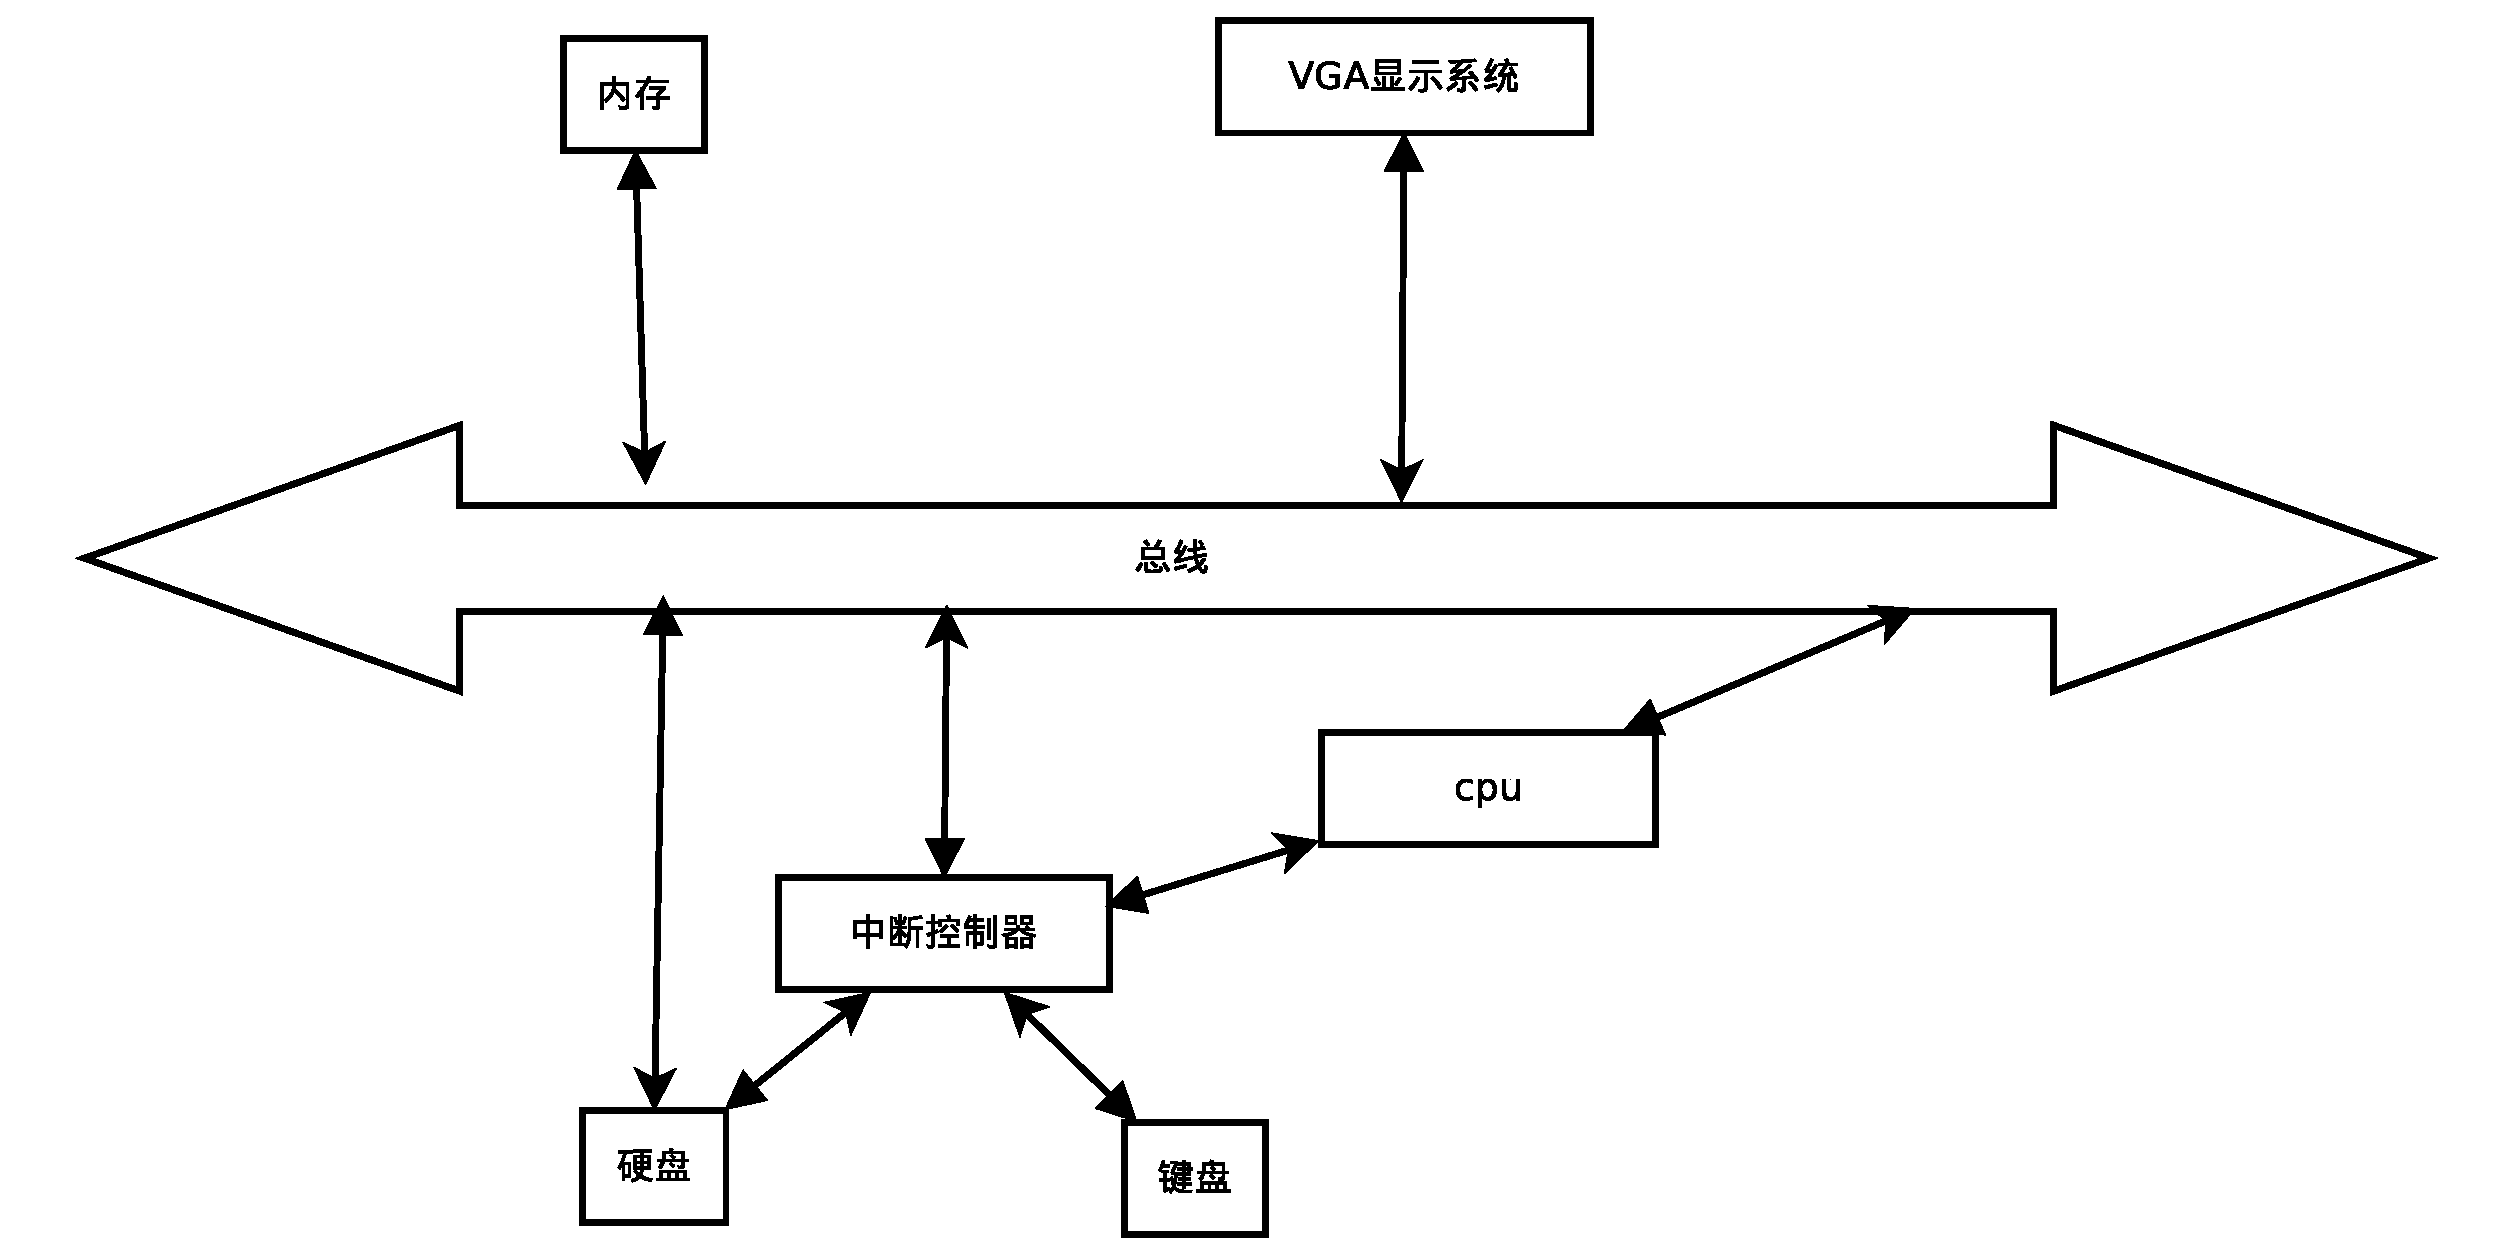
\includegraphics[scale=0.38]{sumti.eps}
\caption{IA32硬件模型}
\label{hard}
\end{figure}

本设计所设计的操作系统针对典型的冯诺伊曼计算机。使用总线结构,系统的各部分组件经由总线相互关联在一起。完成交换数据,传递命令等功能。
\subsection{存储系统}
该模型使用三层存储层次。风别为高速缓冲存储器、主存储器、辅助存储器。高速缓冲存储器用来改善主存储器与中央处理器的速度匹配问题。大小和容量对于系统程序员而言是透明的。主存储器是计算机运行时,存储程序和数据的主要场所。在本设计的模型中其大小为32MB.而辅助存储器用于扩大存储空间。本设计的硬件模型主要有两种类型的辅助存储器。一种是1.44MB大小的软盘。另外一种是ATA硬盘(其大小不固定)。                                                                                     
\subsection{输入输出系统}
像一般的计算机系统一样。该模型使用键盘作为标准输入,也是唯一的输入设备。而将显示器作为输出设备。其中在本设计假设显示系统为典型的VGA系统。
\subsection{中央处理器}
中央处理器是计算机硬件模型的核心部件。是程序运行的地方。本设计的模型使用32位的Intel-80386CPU。而对于设计操作系统而言本设计更关心的是他的寄存器环境。图\ref{80386}展示了80386的寄存器概况。

\begin{figure}[htp]
\centering
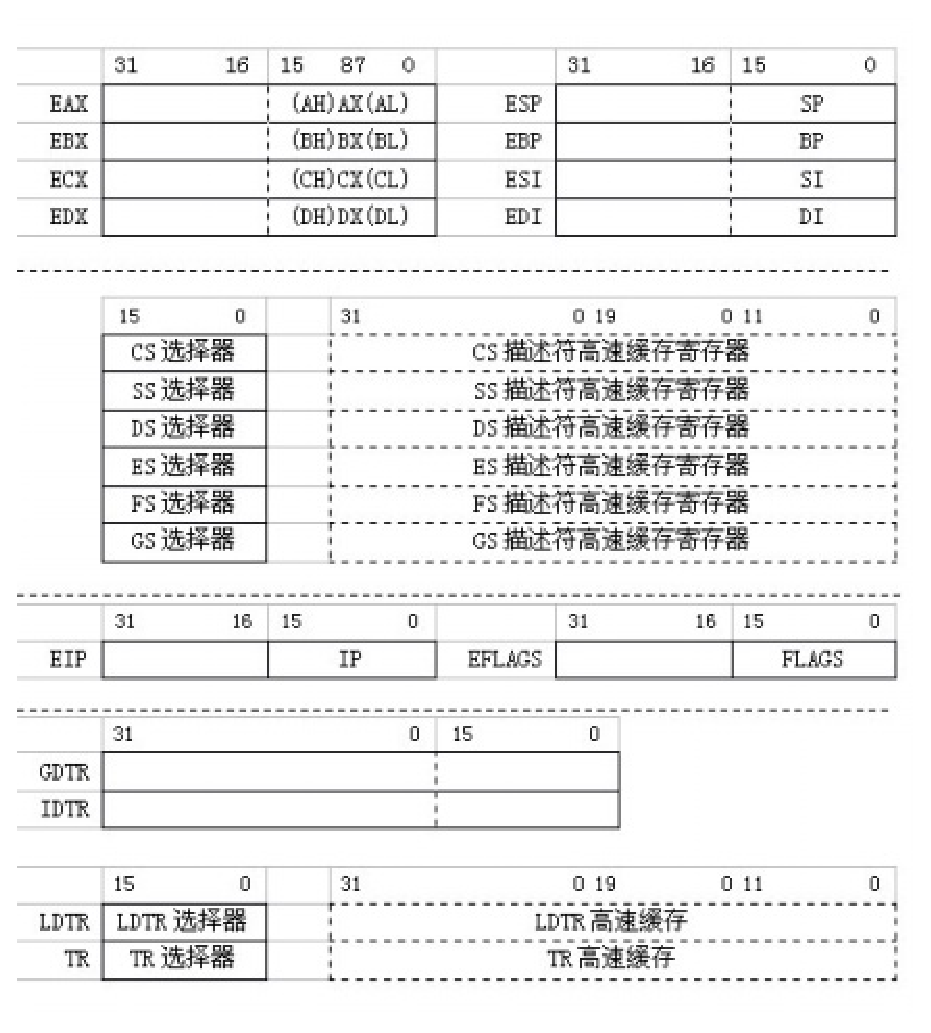
\includegraphics[scale=1]{80386.eps}
\caption{80386寄存器概况}
\label{80386}
\end{figure}


\subsection{中断机制硬件基础}
现在的计算机硬件系统,为了提高信息交换的效率大都采用了中断。采用了中断后,CPU无需空转去等待某个事件的发生。当某个事件发生时向CPU发出一个中断请求信号即可。中断一般用来进行同步操作、实现实时处理、故障处理等功能。而在本设计所设计的操作系统中,中断充当了一个浓墨重彩的角色。硬件系统通过两个中断控制器(主8059A、从8259A)接受来自键盘、硬盘等的各种事件信息,并交付给操作系统处理。图\ref{interrupt}展示了本设计所使用的硬件模型中的中断系统的硬件部分。
\begin{figure}[htp]
\centering
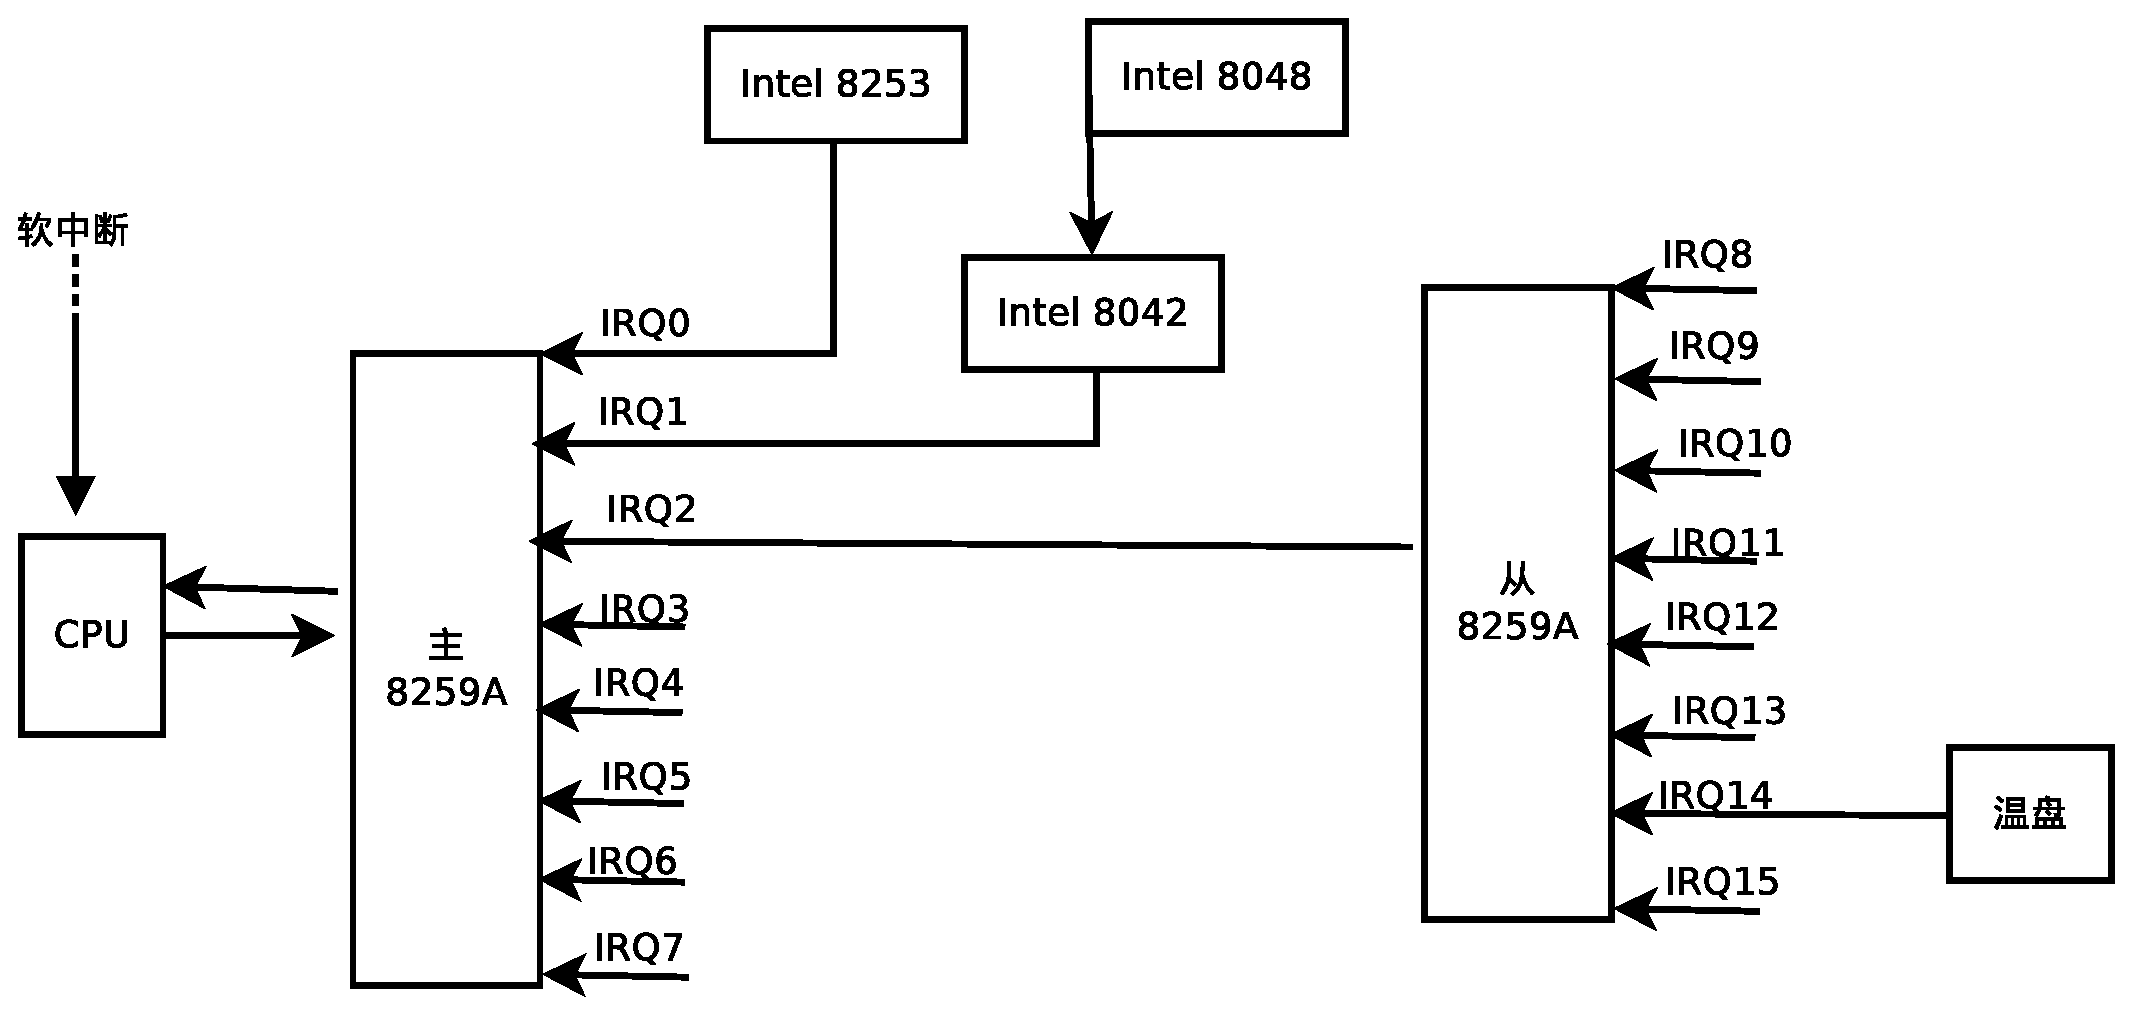
\includegraphics[scale=0.38]{interrupt.eps}
\caption{中断控制器}
\label{interrupt}
\end{figure}

\section{系统启动顺序}
当计算机电源被打开时,他会先进行家电自检(POST),然后寻找启动盘。在本设计所设计的系统中,将启动盘设置为软盘。计算机将会检查软盘的0面0磁道1扇区。如果他以0xAA55结束,则BIOS将其识别为一个引导扇区,并将这512B的内容复制到内存地址0000:7c00处,然后跳转到0000:7c00处将控制权彻底交给这段引导代码。到此为止,计算机将不再由BIOS中固有的程序来控制,而变成由本设计所设计的错做系统的一部分来控制。
\paragraph{}
\indent \ \ 
由于存储介质的限制,一般操作系统的引导信息只能存储在前512B之内。因此本设计不能将一个完整的操作系统内核安放在这非常小的512B之内。因此本设计需要一个专门的程序来引导内核,本设计称这个程序为loader。而且在加载内核之前,本设计还需要设置好内核的运行环境(内存环境和相应寄存器环境),以及为内核准备一些数据。这些工作也又loader来完成。这样下来,一个完成后的loader所占用的存储空间将超过512B,因此也不能安放在那512B的引导扇区之上。于是本设计又需要编写一个程序来引导loader,本设计称这个程序为boot。而在加载完成内核之后,才能够运行各种用户程序。于是本设计所设计的操作系统的引导顺序如图\ref{start}所示。

\begin{figure}[htp]
\centering
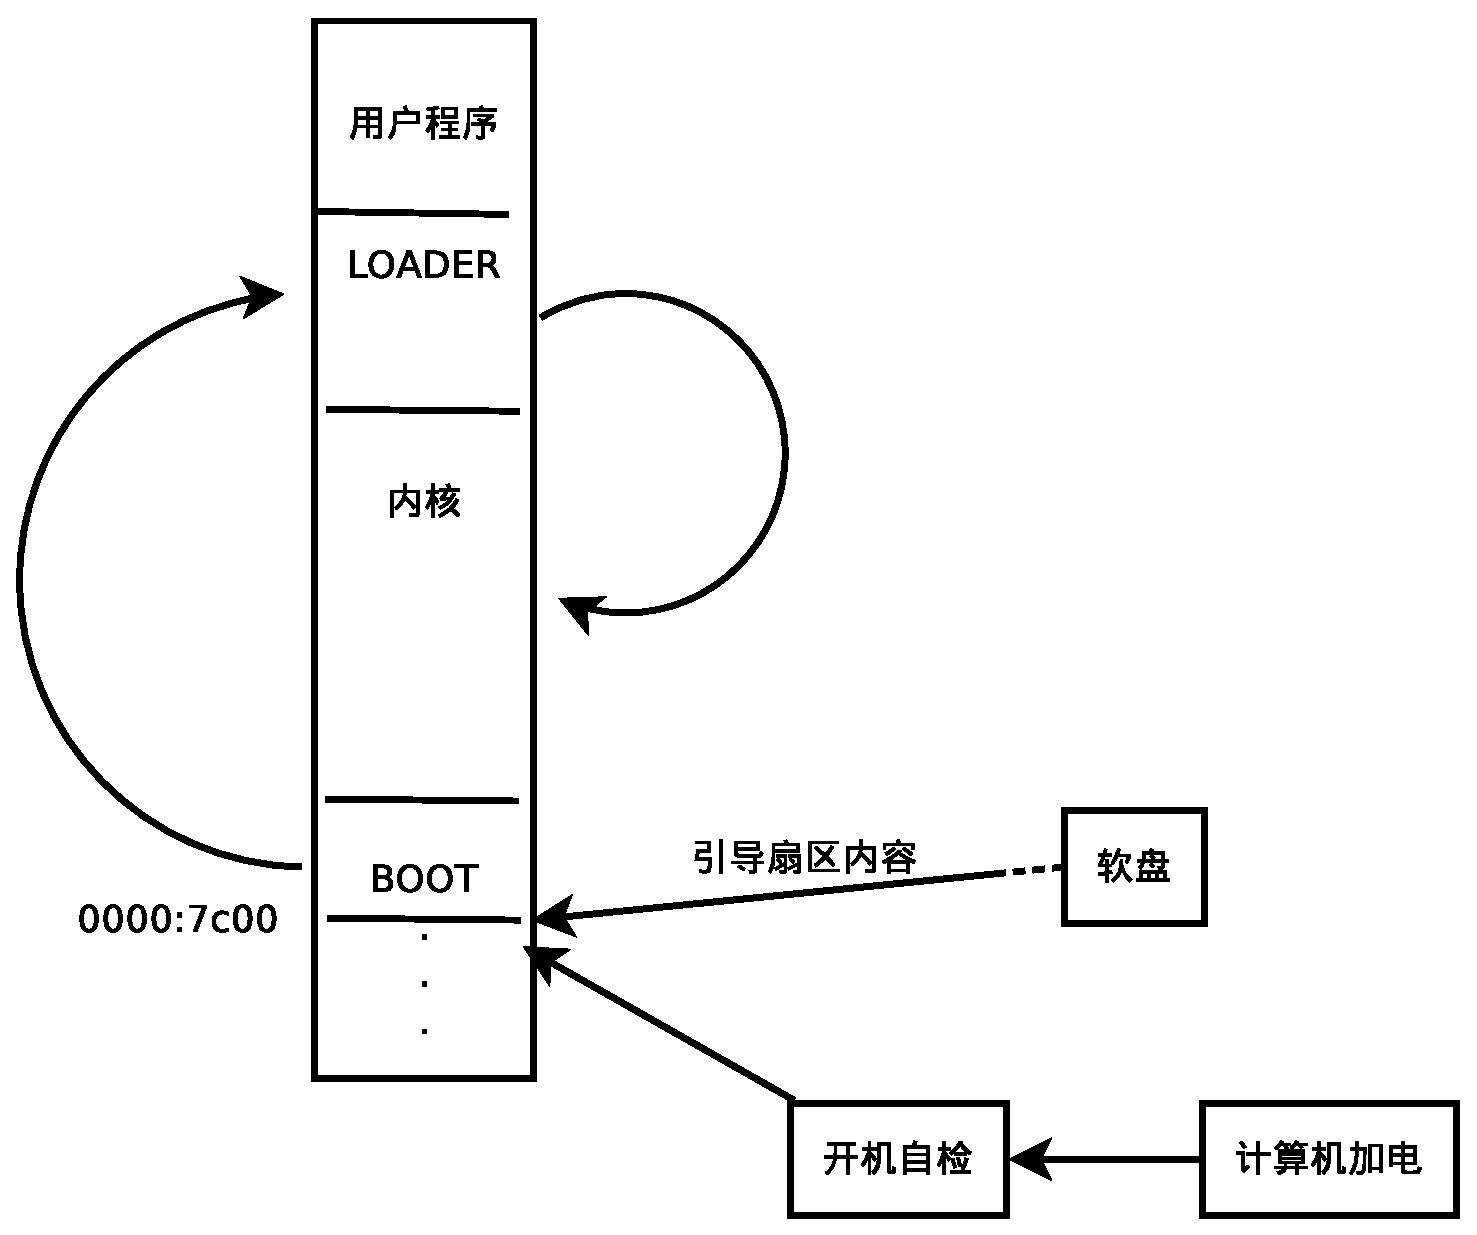
\includegraphics[scale=0.38]{start.eps}
\caption{操作系统启动顺序}
\label{start}
\end{figure}

\subsection{Boot引导程序}
本设计将作为启动介质的软盘做成FAT12格式,以方便操作和查找数据。而Boot模块所要做的,就是从FAT12格式的软盘中将Loader模块的执行文件“LOADER.bin”找出来,并加载到内存的指定位置。
\subsection{Loader加载程序}
Loader完成的功能相对于Boot来说要更加复杂。除了要在存储介质软盘中寻找kernel.bin并将其加载到制定位置外。还要为内存的运行进行一些准备工作。这些工作包括,准备基本的段页式内存管理机制,启动保护模式。
\paragraph{}
\indent \ \ 
系统内核是一个大型的程序,它将会有很多模块组成。而每个模块可能要放到指定的内存地址上。于是Loader必须能够从kernel.bin中解读出哪些程序应该放在哪个特定的位置。于是本设计将kernel.bin链接成ELF(Executable and Linking Format),可执行链接格式。一方便loader解读这些信息。于是Loader从软盘中查找到kernel.bin之后将会对其按照ELF格式进行解读,并合理安放各程序的位置。

\section{内核结构}
本设计所设计的操作系统将提供操作系统的一般功能:进程管理机制,中断服务系统(包括系统调用)、内存管理机制、文件系统、基本的输入输出功能。这些功能各自之间相互独立又相互依赖,共同为用户程序的执行提供软件基础。
\paragraph{}
\indent \ \ 
在比较了宏内核结构和微内核结构的优劣之后。本设计选择了结构更加清晰的微内核结构。微内核结构是一种能够提供必要服务的操作系统内核;其中这些必要的服务包括进程管理,交互进程通信(IPC,Inter-Process Communication)等等。所有服务(包括设备驱动)在用户模式下运行,而处理这些服务同处理其他的任何一个程序一样。因为每个服务只是在自己的地址空间运行。所以这些服务之间彼此之间都受到了保护。微内核是内核的一种精简形式。将通常与内核集成在一起的系统服务层被分离出来,变成可以根据需求加入的选件,这样就可提供更好的可扩展性和更加有效的应用环境。使用微内核设计,对系统进行升级,只要用新模块替换旧模块,不需要改变整个操作系统。于是本设计所设计的操作系统的结构看起来像图\ref{osstruct}所示。
\begin{figure}[htp]
\centering
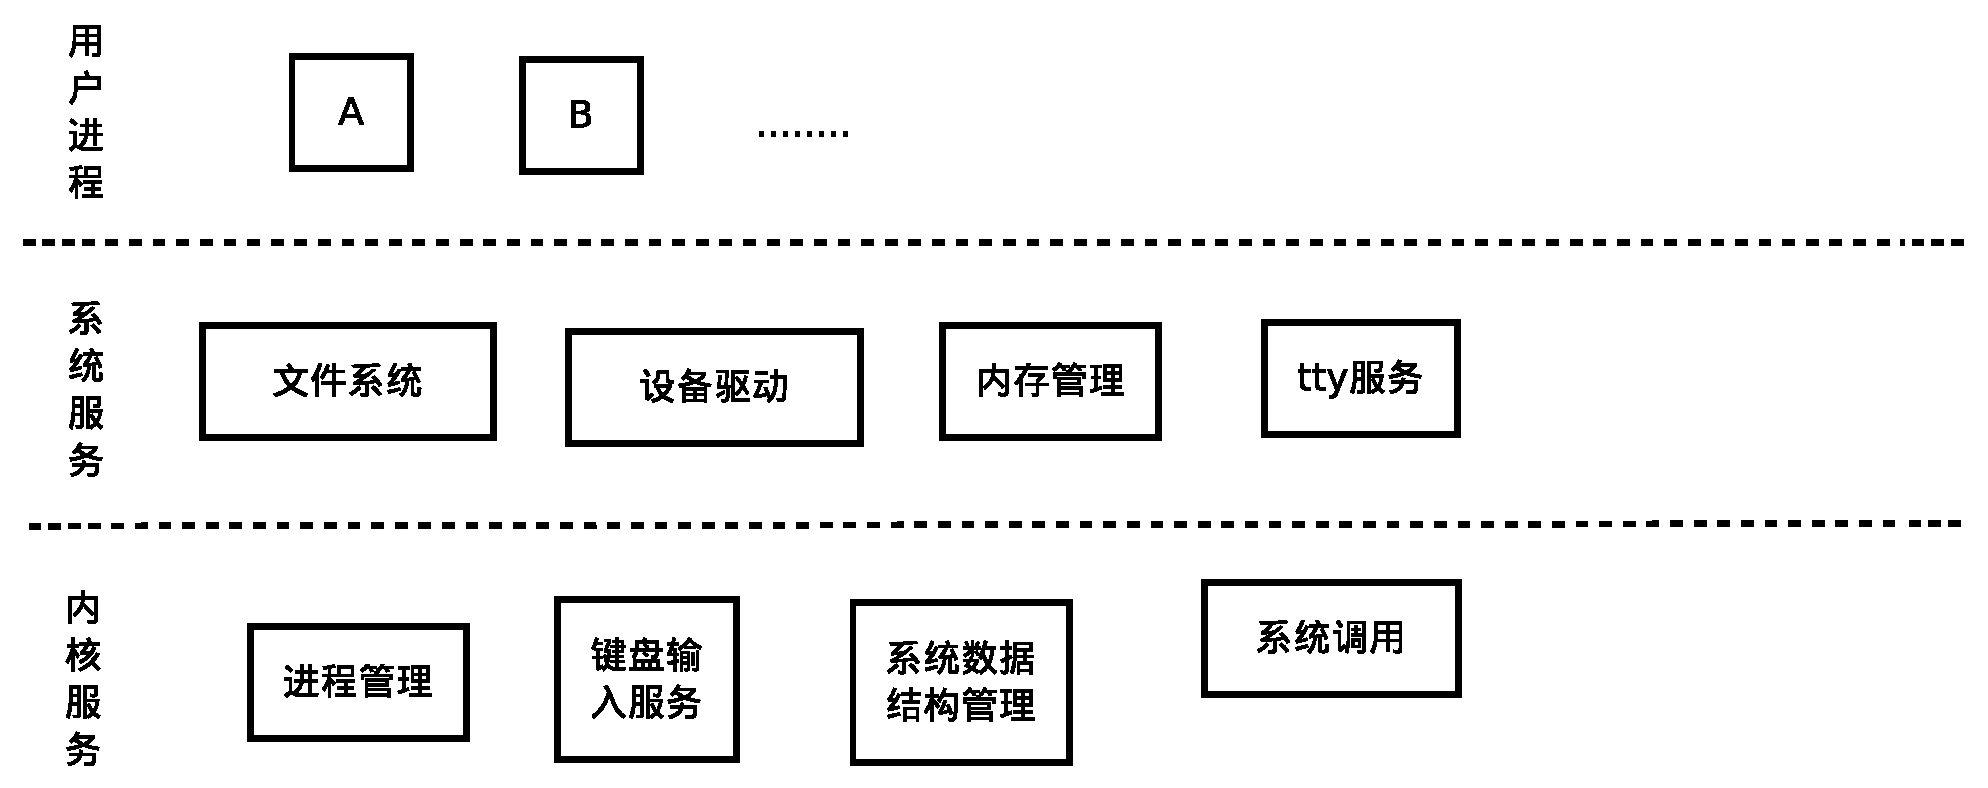
\includegraphics[scale=0.38]{osstruct.eps}
\caption{内核结构}
\label{osstruct}
\end{figure}

\chapter{进程管理}
\section{进程管理服务框架}
进程管理是操作系统非常关键的一部分,它的设计和实现直接影响到整个系统的功能和性能。在一个多进程的操作系统中,一个时间段内可以有多个进程“并发”执行。这样就避免了较为快速的CPU等待较为低速的I/O设备的情况,提高了CPU利用率,从而提高系统的性能。另一个方面,同时运行多个进程,就可以同时提供多种服务或者同时为更多的客户服务,这也是现代操作系统的基本特征。所以只有在设计好进程管理功能的基础上,才能合理分配系统的资源,提高系统的效率。一个程序可运行多次,它的每个运行副本都有自己的进程。同时,一个程序被加载入内存成为一个进程直到他从内存中被移除而死亡的这个过程叫做进程的生命周期。一般一个进程的生命周期包括进程的创建、进程因调度而执行和进程的结束三个步骤。进程并非是自生自灭的。他的生命周期受到操作系统的管制。也就是说操作系统负责着进程的创建、进程的调度、进程的撤销还有分配进程所需要的资源。当然进程在这个生命周期内,因为遇到各种事件而存在着存在着不同的状态。操作系统还要管理处在各种状态下的进程,并对他们进行合理的调度。
\paragraph{}
\indent \ \ 
调度主要有两个问题,一个问题是应该在什么样的时刻或者说当哪个特定的事件发生时就进行调度。第二个问题是进程进程间切换。对于第一个问题本设计使用时间作为衡量标准,每个进程会分得一段时间的CPU使用权限,时间片用完后释放使用权限。当然发生中断的时候实际上,进程也进行了“调度”,只不过这种调度不同于一般的进程调度。对于进程间切换,每一个进程都有自己独特的运行环境(内存环境和寄存器环境等等),都有自己独特的代码、数据、和堆栈,当他因为调度而失去CPU使用权限的时候,操作系统就需要记录下他们独特的运行环境信息。也要为新的进程准备它独特的运行环境。于是进程管理由进程控制块(PCB)、进程调度、中断处理、定时器、进程通信等部分组成。
\section{进程控制块PCB}
%此处先介绍PCB然后是实现
操作系统文献中所提到的PCB的一种实现(在以后的论述中本设计依旧使用PCB的概念来指代proc数据结构)。PCB是进程实体的一部分,是操作系统中最为重要的记录型数据结构,也是操作系统实现进程管理的核心结构。PCB的作用就是使一个在多道程序环境下不能够独立运行的程序(含数据),成为一个能够独立运行的基本单元,一个能够与其他进程并发执行的进程。或者说PCB在操作系统中就代表了一个进程,操作系统施加在进程上的操作都是通过改变进程对应的PCB来实现的。例如,当操作系统要调度某进程执行时,要从该进程的PCB中读取这个进程的状态和优先级;在调度到某进程的时候,要根据其PCB中的处理机状态信息,设置该进程的运行环境。因而需要首先阐述一下在本设计的操作系统中PCB的具体结构。为了描述和控制进程的运行,本设计用一个proc数据结构来表述进程,它包含了进程的详细信息,主要有进程标志(PID)、进程所占用的内存区域、相关文件的描述符、进程环境、信号处理、资源安排、同步处理和进程状态几个方面。proc结构定如下:
\begin{lstlisting}
/*form inclue/sys/proc.c*/
struct proc {
	struct stackframe regs;    /* process registers saved in stack frame */
	u16 ldt_sel;               /* gdt selector giving ldt base and limit */
	struct descriptor ldts[LDT_SIZE]; /* local descs for code and data */
    int ticks;                 /* remained ticks */
    int priority;
	/* u32 pid;                   /\* process id passed in from MM *\/ */
	char name[16];		   /* name of the process */
	int  p_flags;              /**
				    * process flags.
				    * A proc is runnable iff p_flags==0
				    */
	MESSAGE * p_msg;
	int p_recvfrom;
	int p_sendto;
	int has_int_msg;           /**
				    * nonzero if an INTERRUPT occurred when
				    * the task is not ready to deal with it.
				    */
	struct proc * q_sending;   /**
				    * queue of procs sending messages to
				    * this proc
				    */
	struct proc * next_sending;/**
				    * next proc in the sending
				    * queue (q_sending)
				    */
	int p_parent; /**< pid of parent process */
	int exit_status; /**< for parent */
	struct file_desc * filp[NR_FILES];
	struct proc* next;
};
\end{lstlisting}
\subsection{处理机状态}
%加进程切换内容
进程之间切换需要保存失去CPU使用权限的进程的处理机状态信息和进程控制信息。其中,处理状态信息主要是由处理机中各种寄存器组成的。处理机在运行的时候,很多的信息是放在寄存器中的。当发生进程切换的时候,所有这些信息都必须保存在PCB中,以便在该进程重新执行的时候,能够从断点处继续执行。这些寄存器包括:包括PC(program counter)、PSW(processor status word,处理器状态字)、SP(stack pointer,栈指针)、PCBP(pointer of process control block,进程控制块指针),以及其他通用寄存器等。
而proc结构中的struct stackframe数据结构的变量regs就是程序运行时各个寄存器的值。
\begin{lstlisting}
/*from /include/sys/proc,h*/
struct stackframe {	
	u32	gs;		
	u32	fs;		
	u32	es;		
	u32	ds;		
	u32	edi;		
	u32	esi;		
	u32	ebp;		
	u32	kernel_esp;	
	u32	ebx;			
	u32	edx;		
	u32	ecx;		
	u32	eax;		
	u32	retaddr;	
	u32	eip;		
	u32	cs;		
	u32	eflags;		
	u32	esp;		
	u32	ss;		
};
\end{lstlisting}。
\section{进程控制信息}
%1、2.。。。改成括号形式
进程控制信息包括:(1)程序和它的数据的内存地址,以便下次调度的时候能够通过PCB找到程序和它的数据;(2)进程同步和通信机制,是指实现进程同步和进程间通信时必要的机制,如消息队列指针、信号量等;(3)资源清单,记录了这个进程从操作系统中分配得到的资源情况,这里主要是指文件;(4)链接指针,它指出了这个进程所在的队列的下一个进程的PCB的地址。
\subsection{进程调度信息}
%加标号
为了完成进程调度及其相关的功能,使程序能够更好的并发执行,操作系统的每个进程的PCB中存储了一些与之相关的信息。其中有:(1)进程状态,说明当前进程正处在一个什么样的状态下,是进程调度时的依据;(2)进程优先级,指明进程获得CPU使用权限的优先级;(3)与进程调度算法相关的一些信息,比如进程已经执行的时间等。
\paragraph{}
\indent \ \ 
在本设计所设计的操作系统中,进程状态定义有以下几种:
\begin{lstlisting}
/* form include/sys/const.h
 *#define RUNNING 0x00  程序运行
 */
#define SENDING   0x02	/* set when proc trying to send */
#define RECEIVING 0x04	/* set when proc trying to recv */
#define WAITING   0x08	/* set when proc waiting for the child to terminate */
#define HANGING   0x10	/* set when proc exits without being waited by parent */
\end{lstlisting}
在本设计所设计的操作系统中的进程可能具有三种基本状态:就绪、执行和阻塞。而上面的代码中这多种状态只是这三种状态因不同的状态而引发的具体情况而已。比如SENDING和RECEIVING是由于进程间同步通信而引发的阻塞状态。WAITING是程序就绪状态。HANGING是在程序执行完成后退出时的状态。这些状态标志在进程管理的一些具体模块中有着十分重要的功能。而这些模块就是通过这些标志,来判断当前进程的状态,并进行相关的操作的。
\paragraph{}
\indent \ \ 
从一个宏观的角度来看,本设计所设计并实现的操作系统中一个进程的状态转移如图\ref{procstatus}所示。

\begin{figure}[htp]
\centering
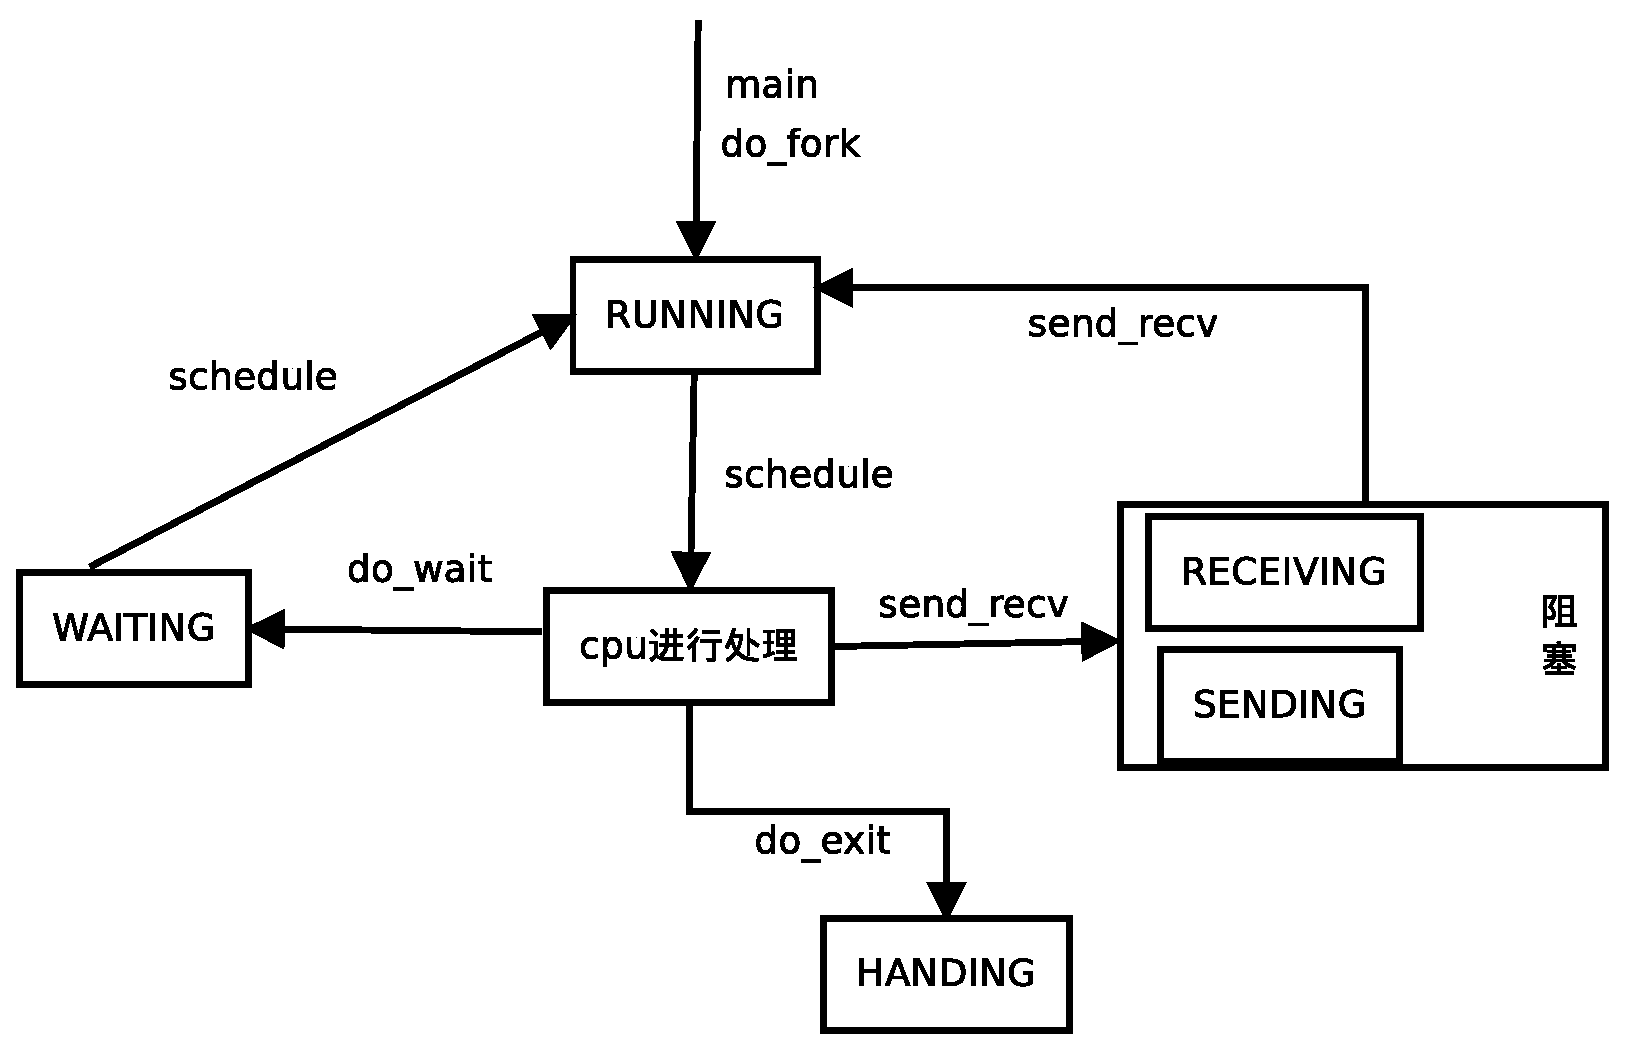
\includegraphics[scale=0.4]{procstatus.eps}
\caption{进程状态转换}
\label{procstatus}
\end{figure}

这里的状态转移主要是针对用户进程而言的。一个用户进程在其父进程使用do\_ dork函数创建这个用户进程后,这个用户进程进入RUUNING状态,经由schdule调度得到cpu使用权开始执行。若在CPU执行过程中需要进行进程间通信或者申请资源得不到的时候将会进入阻塞状态(因阻塞原因不同,会使用不同的标记)。当进程间通信完成或者进程申请的资源被进程得到的时候,将进程状态标记为RUNNING,然后等待shedule调度。当一个用户进程成为了一个父进程要创建其他进程时进程进入WAITING状态。各种过程完成后,将进程状态标记为RUNNING,然后等待shedule调度。
\subsection{进程优先级及进程调度相关}
本设计所设计并实现的操作系统,使用了优先级的概念。程序并不是以相同的机会去获得CPU的使用权限。每个进程在其初始化的时候都有他的优先级。这个优先级代表了程序能够获得CPU使用权限的优先程度。进程控制块中priority代表着进程优先级,进程初始化的时候由系统赋给它一个值,这个值有大有小,代表着进程的优先级。数值越大,优先级越高;数值越小,优先级越小。于是每个进程的运行不再有相等的机会去获得CPU使用权限。在本设计所设计并实现的操作系统中,优先级是一个与时间密切相关的概念。从实质上讲,本设计使用的优先级是种伪优先级机制。程序获得的优先级实质上代表的是他在一次总调度过程中所能够获得的时间片的总数。这个数值越大,程序的优先级越高;数值越小,程序的优先级越小。程序的优先级小的时候,程序会在一次总的调度过程中较早的使用完所有的时间片,然后阻塞。其他没有使用完时间片的进程会继续执行。这样从宏观的角度看来,就像对程序获得CPU使用权限的机会进行了优先级排序。执行在程序初始化时将程序的实时优先级ticks设置成priority的值。每次程序获得CPU使用权限,其ticks值都会减一,当减小到0的时候,程序就失去了获得执行的机会。一直到所有的进程都见到0为止。当所有进程的ticks都为0的时候,进程调度函数会将所有进程的ticks再次设置成它的priority值。并且在进程调度的时候,只有当程序的状态p\_ flags为RUNNING的时候程序才能够获得CPU使用权限。
\subsection{进程通信}
这里所说的进程间通信包括两种机制,一种是同步TIPC机制,另外一直是一种基础的信号量机制。由于本设计所设计并实现的操作系统采用了结构清晰的微内核结构。进程间通信便成了操作系统中一个非常重要的过程。他是各个进程间进行信息交流的依靠。为了保证进程能够及时的收发信息,本设计采用了同步IPC的方式进行进程间通信。并且在进程控制块中设置了相应的数据结构以方便实现这种机制。在每个进程的进程控制块中都保存了一个指向MASSAGE数据结构(消息体)的指针,用以得到进程通信的消息体内容。并且考虑到可能有多个进程参加同一个进程通信过程。在进程控制块中设置了两个指针用以寻找处在发送或者接受链表的下一个或者上一个进程。p\_ recvfrom记录着信息来自哪一个进程。p\_ sendto记录着信息将会发送给哪个进程。
\subsection{进程控制块的组织方式}
在操作系统中,通常会共同存在若干个程序,也就有相应数目的PCB。一般管理这些进程控制块有两种方式,一种是连接方式,把具有同一状态的PCB,连接成一个队列;一种是索引方式,根据系统中进程的各个状态建立几张索引表。而本设计为了能够将它们加以有效的管理,本设计采用了静态数组和链接方式来管理这些PCB。首先在系统初始化的时候建立一个PCB的数组proc\_ table[],它包含了系统中所有的PCB的指针。而且系统中最大进程数受proc\_ table数组大小的限制,默认值为系统预定义的两个常量NR \_ TASKS和NR \_  PROCS之和。而将具有统一状态的PCB,用链接的方式形成队列。这样可以形成就绪队列、若干个阻塞队列和空白队列等。同时也可以根据进程阻塞的原因不能而将进程链接在一起形成一个队列。这种链接方式是通过一个表示进程状态的PCB指针和PCB内部指向其他PCB结构的指针来实现的。
\section{进程的创建与撤销}
进程的创建和撤销是进程控制的主要内容。他用于创建一个新的进程,终止一个已经完成任务的进程,或者去终止一个因出现某事件而使其无法继续运行下去的程序,还可负责进程运行中的状态转换。如当一个正在执行的进程因为某些事件而不能继续执行的时候,将其转化为阻塞状态,而当出现该进程所期待的事件后,又将改进成转换为就绪状态等等。这部分功能由操作系统的内核来完成。
\paragraph{}
\indent \ \ 而操作系统中运行的进程可以分成两类。一类是任务即系统进程,用来提供系统服务,像提供基本输入输出功能的TTY任务。而另外一类是用户自己的程序,是运行在操作系统之上的用户程序。两类进程完成着不一样的功能。因而,对于这两类程序,进程的创建和撤销都有着不一样的过程。一般任务在系统启动的时候由操作系统完成初始化,当操作系统关闭时自动撤销。它的生命周期与操作系统相同。而用户程序则是由各自的父进程创建,并由父进程来撤销并收回其占用资源。用户进程的生命周期收到它的父进程和本身功能的限制。
\subsection{任务的创建和撤销}
任务的主要功能是用来提供系统服务,是操作系统自始至终都在运行着的服务性质的进程。这些进程自始至终都驻留在内存之中,并发执行。他们是操作系统最为关键的部分。于是这些任务的的创建过程也是操作系统启动的一部分,即随着操作系统的启动而创建。随着操作系统的关闭而撤销。任务的创建和撤销完全不需要用户来干预,由操作系统自动完成。在操作系统中,本设计定义了六种任务。他们是系统的基本服务。包括文件系统,硬盘驱动,基本输入输出,内存管理和一种信号量机制。
\begin{lstlisting}
/*from kernel/global.c*/
/* 注意下面的 TASK 的顺序要与 const.h 中对应 */
PUBLIC	struct task	task_table[NR_TASKS] = {
	/* entry        stack size        task name */
	/* -----        ----------        --------- */
	{task_tty,      STACK_SIZE_TTY,   "TTY"       },
	{task_sys,      STACK_SIZE_SYS,   "SYS"       },
	{task_hd,       STACK_SIZE_HD,    "HD"        },
	{task_fs,       STACK_SIZE_FS,    "FS"        },
	{task_mm,       STACK_SIZE_MM,    "MM"        },
    {task_signal,	STACK_SIZE_SIGNAL, "SIGNAL"   }};
\end{lstlisting}
这些任务的初始化工作是在操作系统加载内核的过程中完成的。在这个过程中初始化了任务的PCB中的各个参数并分配了内存和其他资源。使任务能够正常运行。
\begin{lstlisting}
\end{lstlisting}
\subsection{用户进程的创建}
用户进程,是用户用来完成指定的功能的一个程序的运行过程。用户进程,是使用操作系统的编程接口编写而成的对计算机进行管理或者实现功能的程序。而且运行在用户空间之内,并收到系统内核的管理和调度。用户进程一般是用户使用的时候创建,而在完成所应该完成的任务后撤销。这个过程是由该进程的父进程控制完成。每一个用户进程都会经历这样的一个受到父进程控制的生命周期。于是本设计在系统启动的时候就需要创建一个所有用户进程的祖先进程,以创建和撤销其他的进程。这个进程就是init进程。这种方式本设计参考了Linux系统产生其他所有进程的方式。让init进程以守护进程的方式存在。它是系统中所有用户进程的祖先。它负责着本设计所设计并实现的操作系统中用户进程的控制。先面的代码中是用户进程的PCB的定义。
\begin{lstlisting}
/*from kernel/global.c*/
PUBLIC	struct task	user_proc_table[NR_NATIVE_PROCS] = {
	/* entry    stack size     proc name */
	/* -----    ----------     --------- */
	{Init,   STACK_SIZE_INIT,  "INIT" },
	{TestA,  STACK_SIZE_TESTA, "TestA"},
	{TestB,  STACK_SIZE_TESTB, "TestB"},
	{TestC,  STACK_SIZE_TESTC, "TestC"}};
\end{lstlisting}
作为所有用户进程的父进程的init进程所完成的工作主要是创建了一个标准的shell,用以接受用户命令。而接受到用户命令之后调用系统调用exec来完成进程的创建。在用户进程完成任务后,发送消息给父进程,父进程通知内存管理程序撤销该用户进程。系统调用exec的语义很简单,它将当前的进程映像替换成另一个。也就是说,本设计从硬盘上读取另外一个可执行文件,用它替换掉被从Init创建出来的新进程。这样一来被替换的子进程就摇身一变成了一个彻头彻尾的新进程。这个过程说起来很简单,但是真正实现起来却比较麻烦。因为一个新进程诞生时,需要从系统中分配一些资源,比如关键的内存。于是init进程要和其他的管理模块进行交互,其中最为关键的就是内存管理模块。
\paragraph{}
\indent \ \ 在系统启动的时候,本设计已经初始化好了所有的进程PCB,包括把每一PCB的LDT选择子和GDT表项准备好,并且在proc\_ tabel[]中预留出了一些空项供新进程使用。并将部分PCB的p\_ flags设置为FREE\ SLOT表示这个PCB是空项,没有指示任何具有实际意义的进程。在系统调用exec中首先调用fork函数。fork函数回向内存管理进程发送一个FORK信息,最终内存管理进程调用do\_ fork()函数如附录\ref{dofork},进行一些进程PCB的设置。首先是分配进程表。在数组proc\_ table中寻找一个空项,用于存放子进程的进程表。然后分配内存。由于子进程是父进程的副本,所以需要首先获得父进程的内存占用情况,这由读取父进程的LDT来完成。然后将父进程的内存空间完整的复制一份给子进程新分配的空间。然后是通知文件系统模块,因为父进程和子进程之间可能要共享文件。之后函数返回,并发消息给内存管理模块。
\paragraph{}
\indent \ \ 之后发送EXEC消息给内存管理模块,让进程真正运行起来。内存管理模块接受到EXEC消息后,最终调用do\_ exec函数。从消息体中读取刚刚获得的内存分配信息。并使用系统调用stat()获得程序文件大小。之后将程序文件读入内存的缓冲区中。并根据ELF文件的程序头信息,将被执行文件的各个段放置到合适的位置。之后建立参数栈。为程序的各个相关寄存器赋值,这里关键的寄存器是eax、ecx、eip和esp。其中eax和ecx是程序从shell中获得的参数。eip指向程序的入口地址。esp指向刚刚准备好的堆栈的位置。之后给进程一个名字。程序就运行起来了。
\subsection{用户进程的撤销}
前面已经提到进程在操作系统中是有一个生命周期的。进程有产生就会有消亡。不然进程只产生而不消亡,系统不久之后就会因为资源耗费过度而崩溃。然而,当进程撤销或者说消亡的时候,有些时候只释放资源然后推出就行了,但有些时候该进程还会有子进程。这个时候就有了两种不同的进程撤销函数exit和wait。他们都是向内存管理模块发送消息而最终实现功能。
\paragraph{}
\indent \ \ 
exit最终调用的是do\_ exit函数。这个函数首先告诉文件系统进程要推出,并进行相应的处理。之后释放进程所占用的内存。然后判断P是否正在阻塞。如果是就清除进程的阻塞状态,清除p\_ flsgs的WAITING位。并向进程发送消息接触阻塞。之后释放A的进程表项。如果不是就设置A的状态为HANGING,即挂起。至此,进程完成退出。
\paragraph{}
\indent \ \ wait的功能与exit有点类似。但是却又不同。如果进程S调用wait,那么程序会首先遍历PCB表,如果发现有一个进程A是该进程的子进程,并且这个子进程正在挂起等待退出。那么就向进程S发送消息消息解除阻塞,之后释放A的进程表项,令A退出。如果P没有子进程在挂起,那么就设置P为阻塞。如果P压根就没有什么子进程,则向P发送一个表示出错的返回值。
\section{进程间通信}
\subsection{同步IPC}
IPC是Inter-Process Communication的缩写,直译为进程间通信,说白了就是进程间发送消息。而本设计使用的是同步IPC,它不像寄邮件那样,倒像接力赛,发送者一直等到接受者收到消息才肯放手,接受者也一样,接不消息就一直等着,不干别的。使用同步IPC有若干好处比如:操作系统不用另外维护缓冲区来存放正在传递的消息;操作系统不需要保留一份消息副本;操作系统不需要维护接收队列;发送者和接受者都可在任何时刻清晰且容易知道消息是怎样发送的;从实现系统调用的角度来讲,同步IPC更加合理——当使用系统调用的时候,本设计的确需要等待内核返回结果之后在继续。同时,因为本设计的操作系统所使用的内核结构为微内核结构。这种同步IPC便成了最为关键的一种进程间通信方式。内核中的各个任务和用户的进程都是通过这种同步IPC方式来传递消息。
\paragraph{}
\indent \ \ 
本设计所使用的同步IPC是使用了共享内存的方式来实现的。需要发送消息的进程会创建一个MESSAGE数据结构的共享变量。并用自己将要传递的消息来初始化这个共享变量。之后将这个共享变量共享给希望得到这个消息的进程。这个所谓的共享是通过C语言中的指针实现的。下面将从消息的发送和接受两个方面,来解释一下整个同步IPC机制是怎样运转起来的。
\paragraph{}
\indent \ \ 假设有进程A想向进程B发送消息M,那么过程将会是这样的:
\\ \indent (1)进程A准备好M。
\\ \indent (2)A通过系统调用sendrec,最终调用msg\_ send。
\\ \indent (3)简单判断是否发生死锁。
\\ \indent 4.判断目标进程B是否正在等待来自A的消息:如果是,消息被复制给B,B被接触阻塞,继续运行;如果不是,A被阻塞,并加入到B的发送队列中。
\paragraph{}
\indent \ \ 假设进程B想要接受消息(来自特定进程、中断或者任意进程),那么过程将会是这样的:
\\ \indent 1.B准备一个空的消息结构M,用于接受消息。
\\ \indent 2.B通过系统调用sendrec,最终调用msg\_ receive。
\\ \indent 3.判断B是否有个来自硬件的消息(通过has\_ int\_ msg),如果是,并且B准备接受来自任意中断的消息,则马上准备一个消息给B,并返回。
\\ \indent 4.如果B想要接受来自任意进程的消息,则从自己的发送队列中选取第一个(如果队列非空),将其消息复制给M。
\\ \indent 5.如果B是想接受来自特定进程A的消息,则先判断A时候正在等待发送消息,若是,将其消息复制给M。
\\ \indent 6.如果此时没有任何进程发消息给B,B会被阻塞。
\paragraph{}
\indent \ \ 这样一来整个同步IPC机制的过程就如图\ref{sendrecv}所示:

\begin{figure}[htp]
\centering
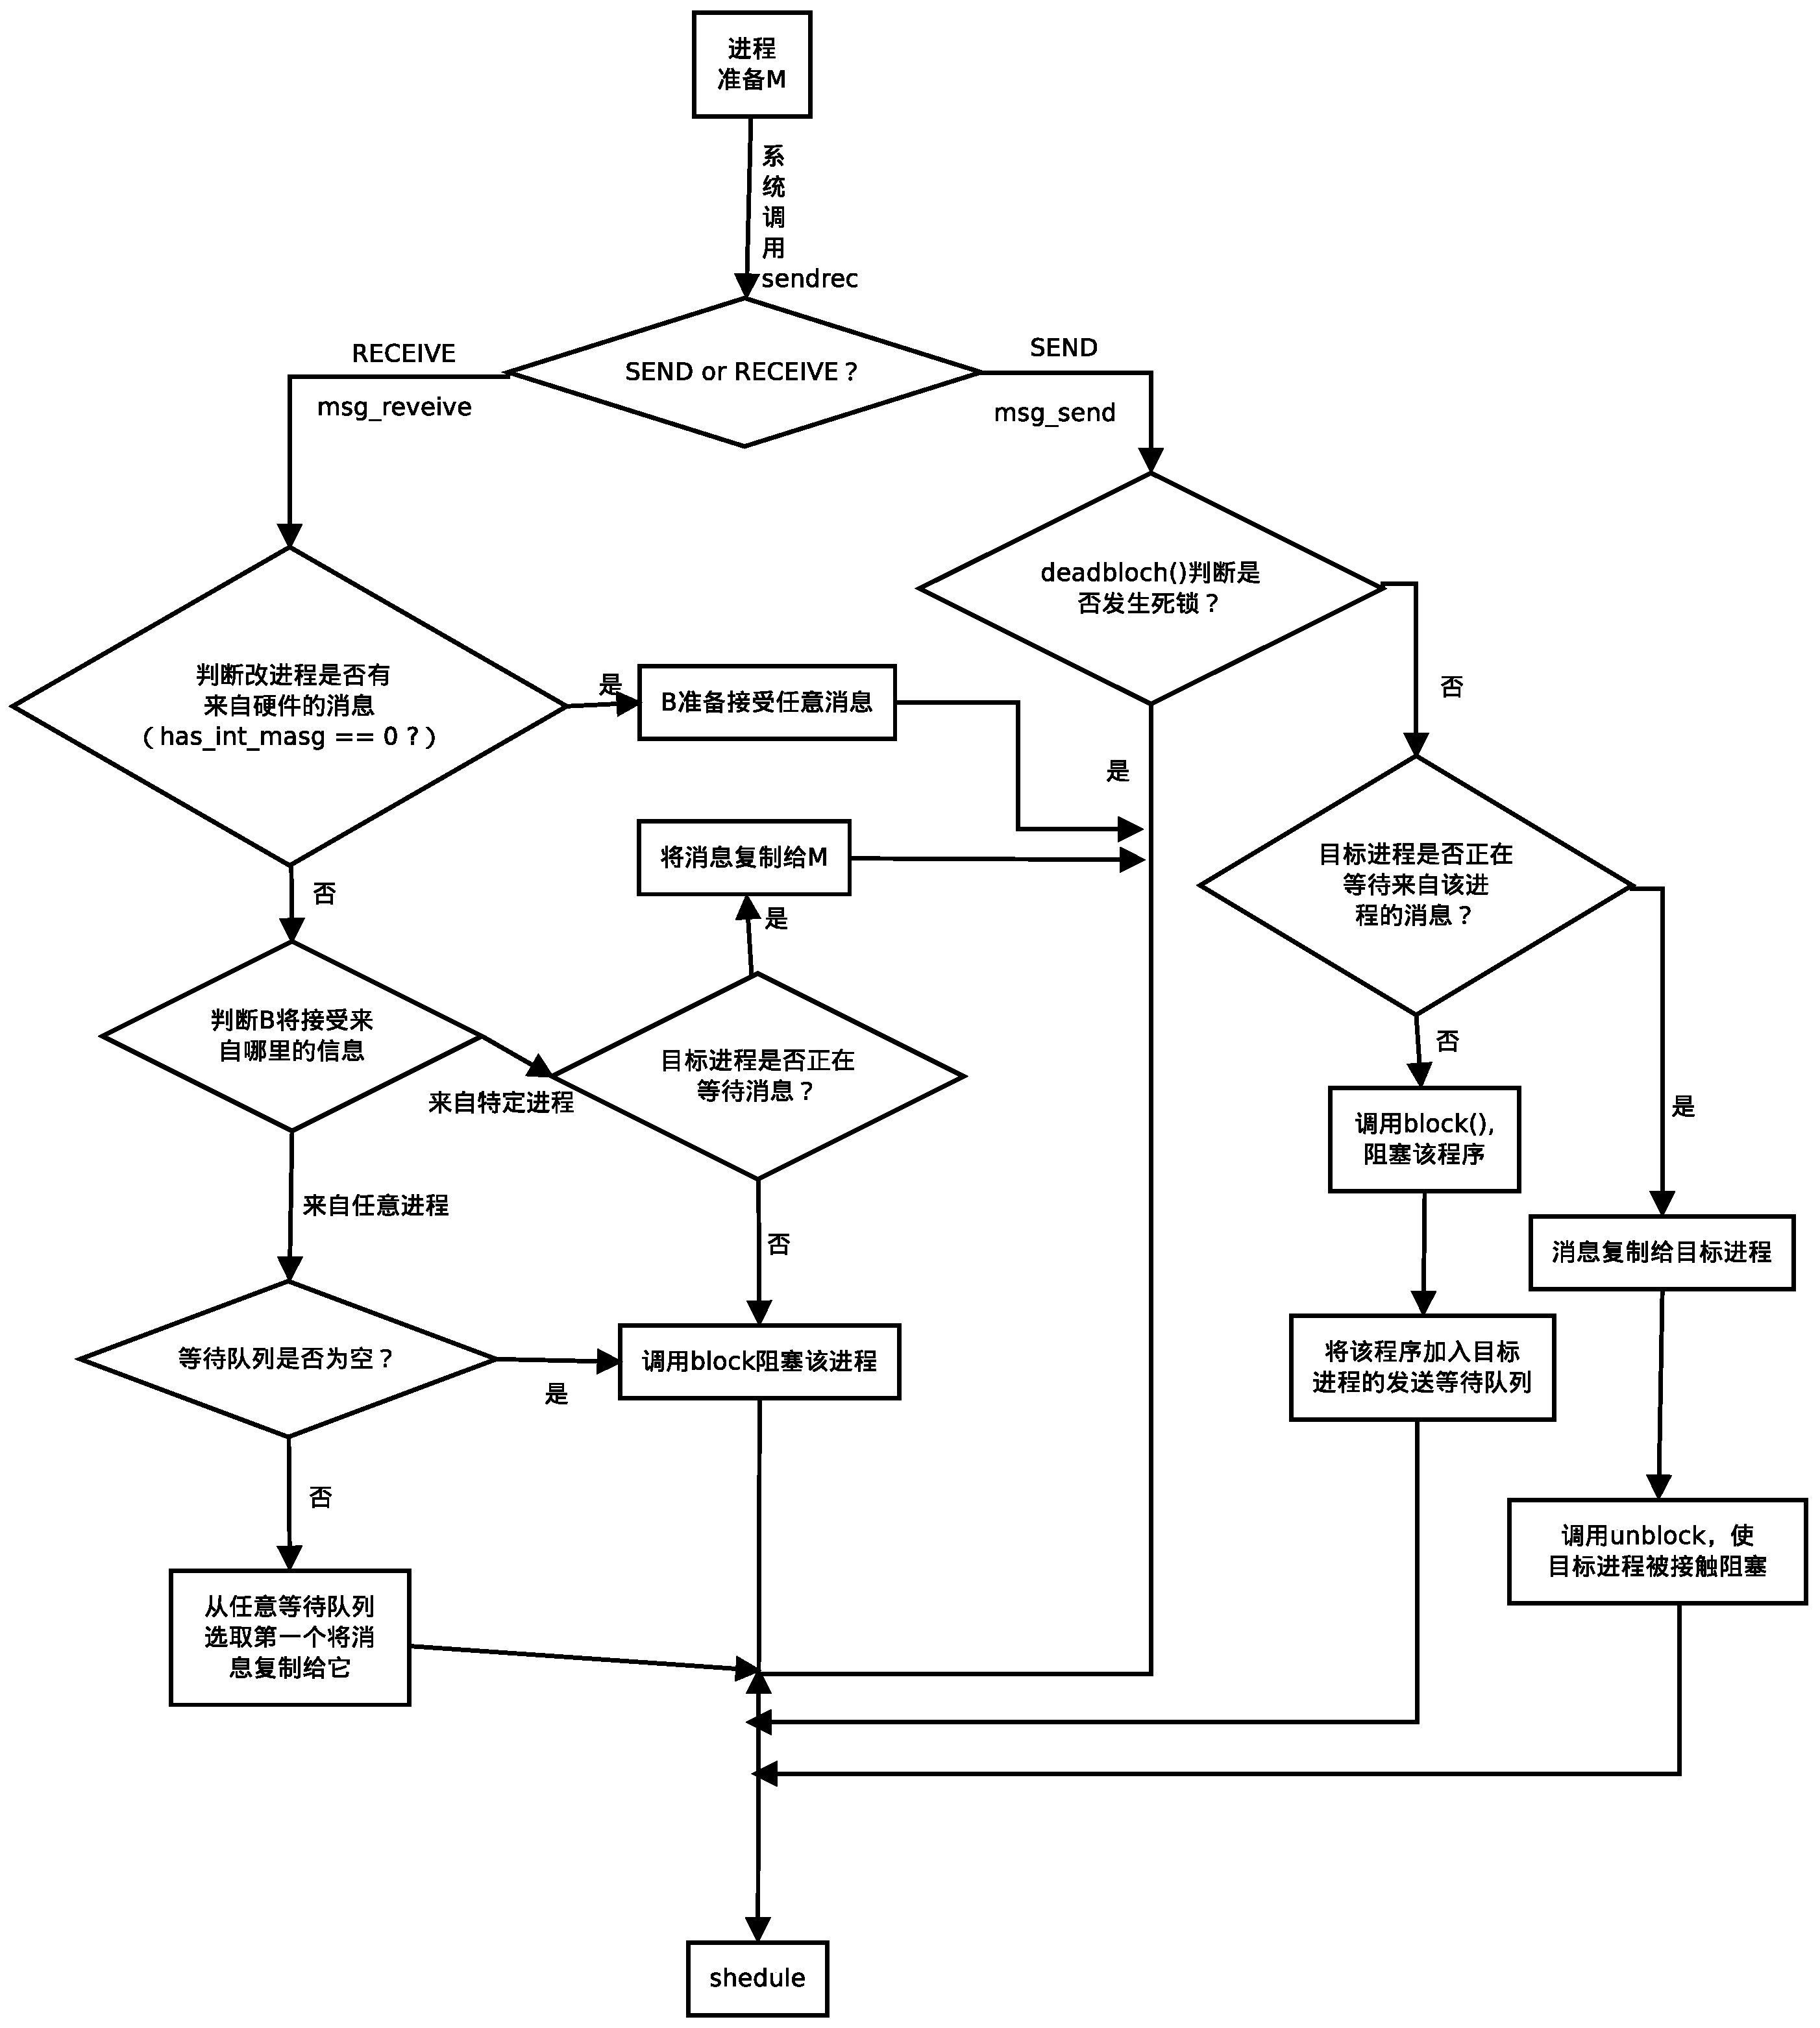
\includegraphics[scale=0.34]{sendrecv.eps}
\caption{进程间通信}
\label{sendrecv}
\end{figure}
\subsection{信号量机制}
在操作系统引入了进程之后,虽然提高了资源的利用率和系统的吞吐量。但由于进程的异步性,也给系统造成了混乱,尤其他们在争用临界资源的时候。例如,多个进程去读写同一个文件的时候,就有可能产生脏数据。而信号量机制的作用就是使诸进程之间能够有效的共享资源和合作,从而使程序更好的执行。信号量机制最早由荷兰学者Dijkstra提出。后来,在长期的应用实践中,信号量机制又得到了很大的发展,它从整形信号量经记录行信号量进而发展成为信号量集机制。而现在信号量机制已被广泛的应用于单处理机和多处理机系统系统以及计算机网络中。本设计所设计的操作系统中的信号量机制继承了信号量集的主要思想。将系统中令进程存在互斥和同步关系的资源和事件全部抽象成临界资源。使用数据结构truct singnaldata来表示临界资源。
\begin{lstlisting}
typedef struct singnaldata{
	int		type;
	int		resource;
	int		limit;
    struct proc*		waitlist;
}semaphore;
\end{lstlisting}
其中三个整形变量与临界资源有关。type代表着临界资源的类型。resource代表系统临界资源的拥有量。而limit则代表着系统最少持有的临界资源的数量。本设计所设计的信号量机制考虑到了这种信号量机制向各种信号量机制的扩展。所以使用了灵活的资源上下限。waitlist是因为此临界资源而阻塞的进程链表队列。本设计依然使用数组的方法来管理所有的临界资源。在系统初始化的过程中,创建了一个全局数组semaphore\_ table[NRSEMAPHORE]用来管理临界资源。数组中的每一个元素都代表了一种临界资源,系统中总共允许存在NRSEMAPHORE(32)个临界资源。系统使用一个系统级的任务来管理所有临界资源,完成对临界资源的操作。下面将介绍一下信号量机制的具体运行过程。
\paragraph{}
\indent \ \ 对于临界资源的操作也是由signal和wait两种相互对立的操作完成。signal用于对释放资源,wait用于申请资源。当用户使用wait操作申请一个临界资源的时候,会经历以下步骤:
\\ \indent 1.遍历semaphore\_ table[NRSEMAPHORE],查看用户申请的临界资源是否注册过。若注册过则转2,否则转3.
\\ \indent 2.检测用户申请的临界资源数量是否小于系统现有数量(resource-limit)。如果是,则分配。如果不是则转4.
\\ \indent 3.注册该资源类型,并将系统现有资源数量置为-1,该临界资源下限置为0。转4.
\\ \indent 4.阻塞进程,并将进程挂入该临界资源的等待队列waitlist中。
\paragraph{}
\indent \ \ 当用户使用signal释放一个临界资源的时候,会经历以下步骤:
\\ \indent 1.遍历semaphore\_ table[NRSEMAPHORE],查看用户申请的临界资源是否注册过。若注册过则转2,否则转3.
\\ \indent 2.将该临界资源的数量增加用户释放的资源量。并从等待队列中取出队首进程,尝试对其进行signal操作,成功则正式分配资源,并唤醒进程。失败则返回。
\\ \indent 3.注册该资源类型,并将系统现有资源数量置为1,该临界资源下限置为0。并返回。


\section{中断管理}
\subsection{中断管理框架}
实时系统要求对具有较高时间要求的活动以及对外来信息要以足够块的速度进行处理,并在一定时间内作出相应,实时系统的最大特点就是实时性,实时系统的中断管理机构是实现实时系统实时相应的机构之一。
\paragraph{}
\indent \ \ 在实时系统中,由于外部事件的不确定性和客观性,受控硬件的各个参数、信息、活动需要处理时,往往向CPU发出中断请求,要求CPU进行处理,中断机制的引入可以让CPU和外设达到真正的并行。并且中断机制也是计算机实现并发的基础之一,中断机制的实现和硬件紧密相连(参见第一章)。在本设计的硬件模型中使用了两个Intel8259A,并使用主从结构相连。系统总共能够处理15种硬件中断。本设计在说到中断的时候往往与异常相提并论。实际上,他们都是程序在执行过程中的强制性转移,转移到相应的处理程序。中断一般是程序执行过程中因为硬件而产生。异常则通常在处理器执行指令过程中检测到错误时发生,比如遇到零除的情况。处理器检测的错误条件有很多,比如保护违例、页错误等。因此所设计的中断机制除了能够响应和处理一般的硬件中断之外,还要能够处理保护模式下的一些异常。
\paragraph{}
\indent \ \ 在多进程的环境中,系统必须对中断进行统一的管理,同时也必须对异常进行统一的管理。从软件的角度出发,对中断的处理分为三个步骤:
\\ \indent 1.中断处理入口的处理。
\\ \indent 2.系统或用户定义的中断服务程序。
\\ \indent 2.中断处理出口的处理。
整个过程正如图\ref{interup}所示。

\begin{figure}[htp]
\centering
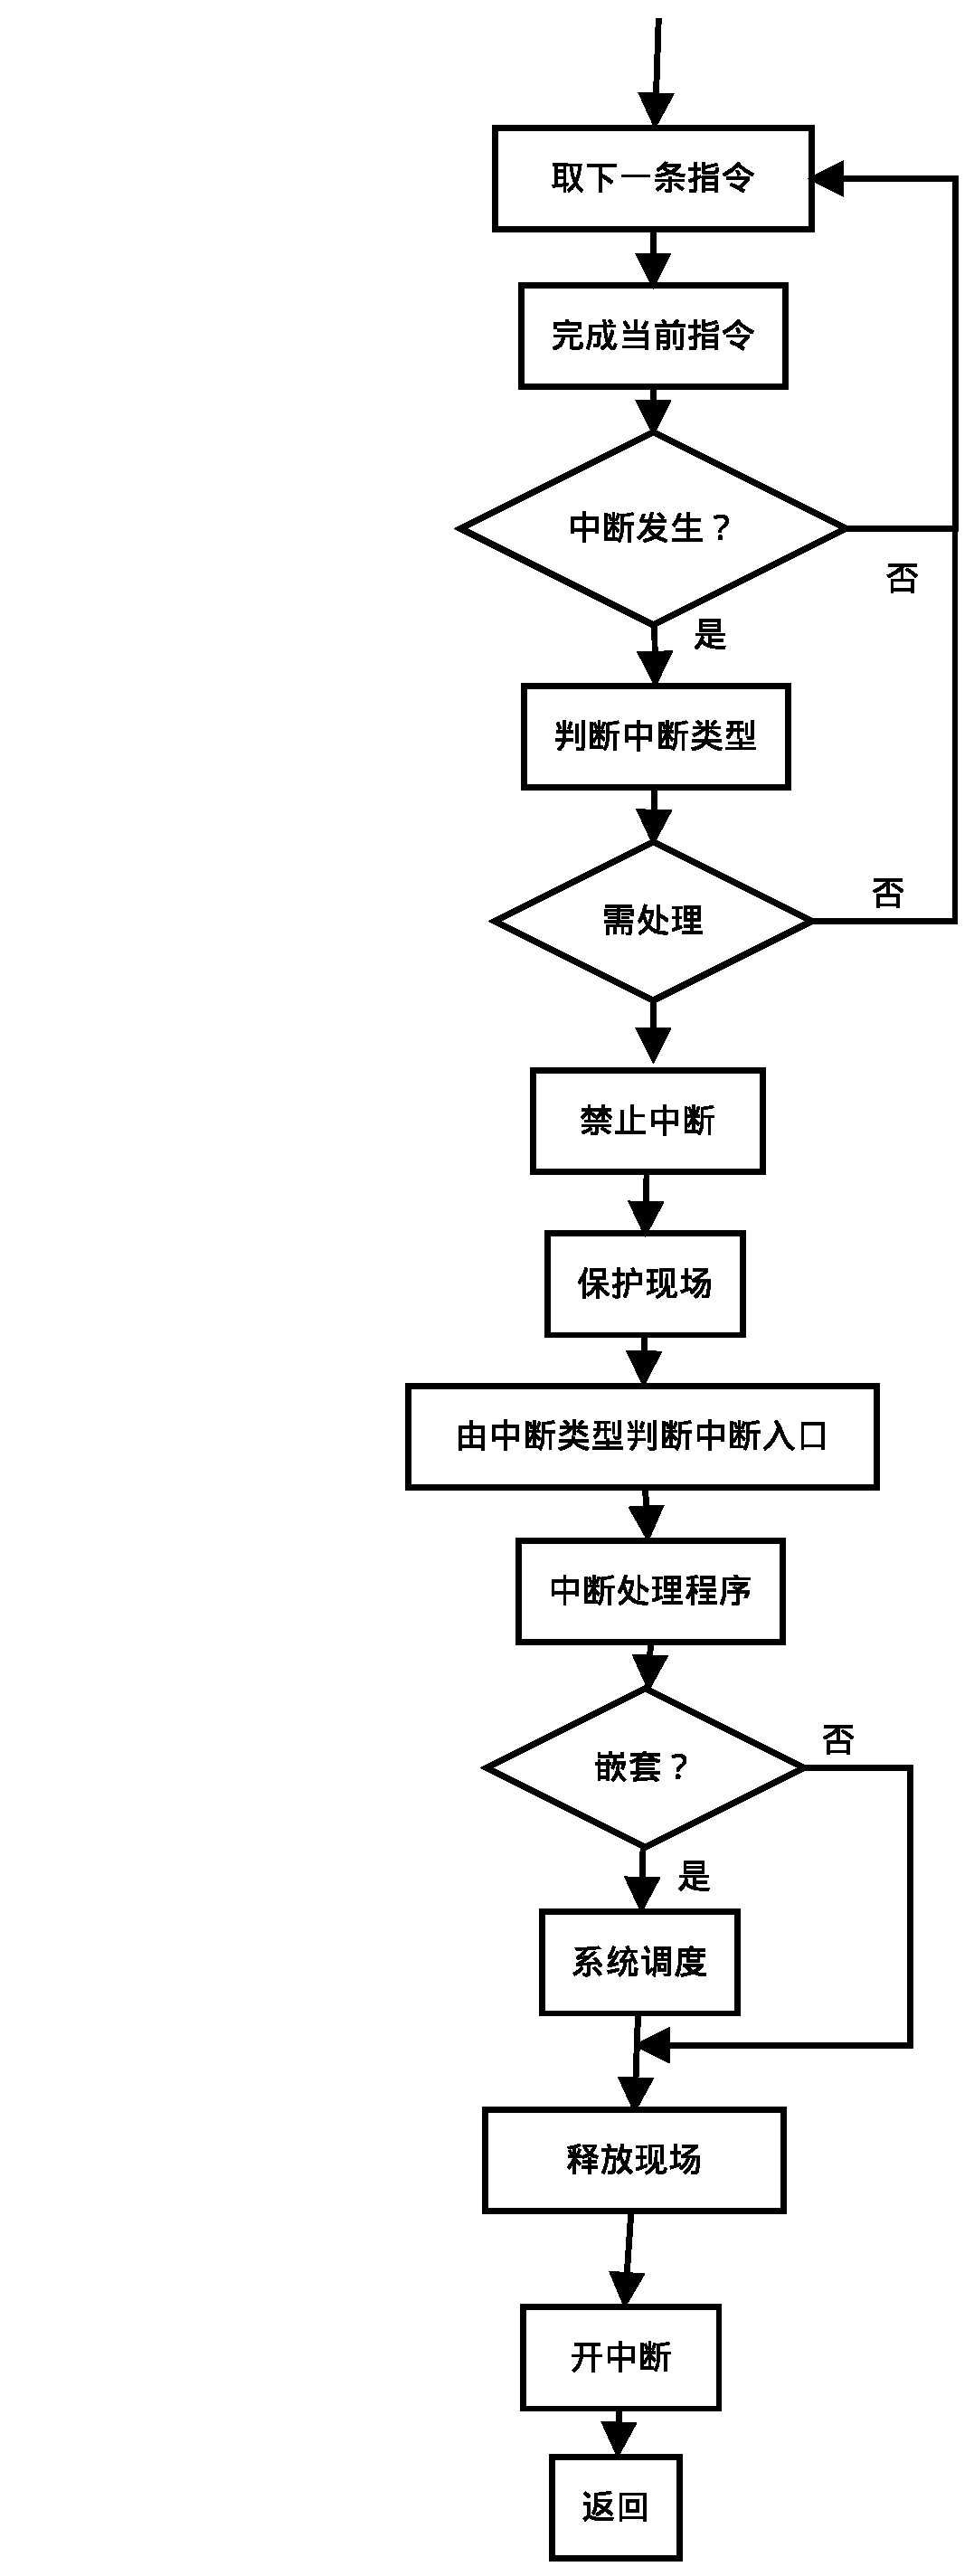
\includegraphics[scale=0.4]{interup.eps}
\caption{中断处理}
\label{interup}
\end{figure}
\indent 中断发生时,硬件根据中断向量进入中断处理入口,该入口不是统一的入口,而是对每一个向量都设置相应的中断类型标志,进入中断总控程序,此程序将所有现场保护进栈后,根据类型标志,转移去执行系统或者用户定义的中断服务程序。
\paragraph{}
\indent \ \ 由于操作系统运行在保护模式下,原来在实模式中实现中断用的中断向量表被IDT(Iterrupt Descriptor Table)所替代。这个表也是个描述符表,叫做中断描述符表。IDT的作用是将每一个中断向量和对应的描述符对应起来。从这个意义上讲IDT也是一种向量表,虽然它在形式上与实模式下的向量表非常不同。于是在保护模式下一次中断处理中寻找相应处理程序入口的过程就变成了图\ref{interruptslove}所示。
\begin{figure}[htp]
\centering
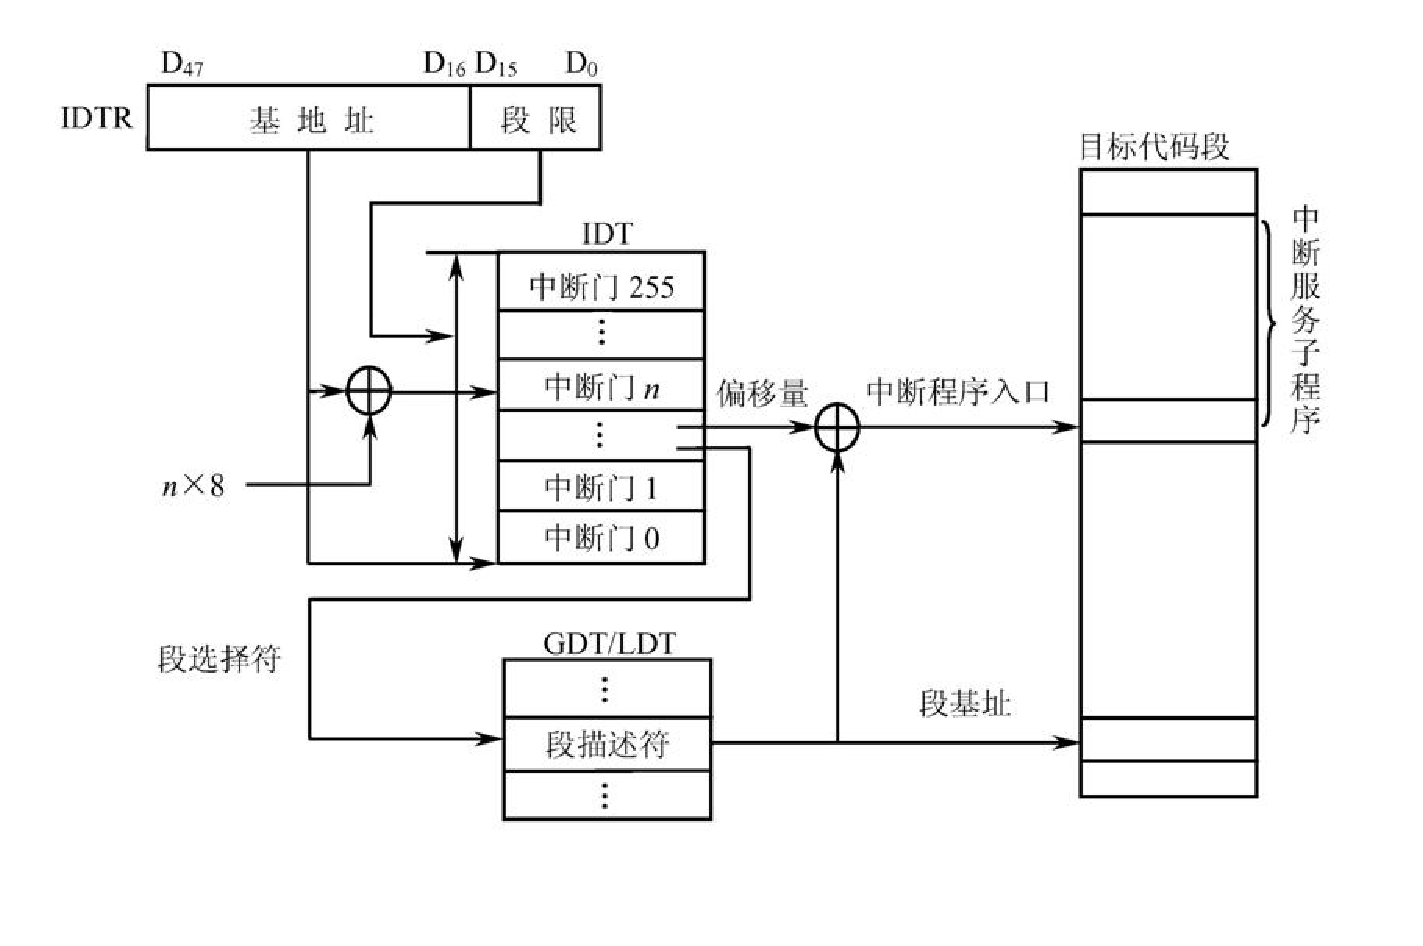
\includegraphics[scale=0.4]{interruptslove.eps}
\caption{寻找中断向量}
\label{interruptslove}
\end{figure}
\indent \ \ 
中断处理出口,首先要检查中断桥套的层次和是否应该调度在局定从哪个出口返回。
\subsection{初始化Inter8259A}
在系统初始化过程中本设计将对两个中断控制器8259A进行初始化工作,并且初始化各种响应和处理中断有关的数据结构。初始化函数首先向主8259A和从8259A发送了相应的状态字和命令字,确定了他们的工作方式。然后初始化了一个函数指针数组irq\_ table,指向各个中断处理程序的入口地址。
\begin{lstlisting}
/*form kernel/global.c*/
PUBLIC	irq_handler	irq_table[NR_IRQ];
\end{lstlisting}
其中irq\_ handler的定义在type.h中:
\begin{lstlisting}
/*form include/type.h*/
typedef	void	(*int_handler)	();
\end{lstlisting}
NR\_ IRQ的值定义为16,以对应主从两个8259A。实际上主从方式的两个8259A只可以处理15种硬件中断,在这个设置成16中只是为了实现上的方便。
\begin{lstlisting}
/*form include/sys/const.h*/
#define	NR_IRQ		16	/* Number of IRQs */
\end{lstlisting}
\subsection{初始化IDT}
中断服务中将中断和异常使用统一的过程来处理,这样既简化了中断服务的逻辑,又方便了实现。系统在启动的过程中初始化了IDT。将所有的中断和异常与他们所对应的处理程序的入口在IDT中设置好。并将所有的异常初始化成中断门,每一种异常的处理函数是不一杨。比如零除异常的处理函数为divide\_ error()。然后本设计配置了中断向量。之后函数填充了堆栈切换事的重要数据结构TSS。同时也初始化了系统调用的入口地址。
\subsection{中断和异常处理}
本设计使用统一的中断处理方式来处理各种各样的中断。即通过中断号选找中断入口程序的方式。这里使用了一个只有一个参数的宏hwint\_ master(从8259A使用hwint\_ slave宏)。比如对于一种时钟中断的处理函数hwint00。本设计将时钟中断的中断号0以参数的形式传递给宏hwint\_ master。在宏hwint\_ master中,首先调用save函数保护现场。然后从函数指针数组irq\_ table中找到相应的中断处理程序函数的入口地址,调用之。之后还原现场,退出中断处理程序。
\paragraph{}
\indent \ \ 而对于异常,本设计则使用了唯一的一个异常处理函数如附件\ref{exception}。函数接受由系统传递来的异常号,然后查找出其对应的异常信息,并将其显示到屏幕上。之后,整个系统宕机。
\section{时钟中断}
本设计所使用的进程角度机制是基于时间片的,也就是说程序在一开始运行的时候确定了进程所能获得的时间片总数,随着运行进程还能够获得时间片总数将会减小。于是时间片大小的确定就非常重要。时间片决定了一个程序一次获得CPU权限的时间是多长。而时间片大小是由时钟中断决定的。中断当然不会凭空产生,实际上它是由一个叫做PIT(Programmable Interval Timer)的芯片来触发的。在本设计的硬件模型中这个芯片使用的是Intel 8253。Intel 8253有三个计数器,本设计使用计数器Counter 0,它的作用是每隔一段时间让系统产生一次时钟中断。计数器的工作原理是这样的:它有一个固定的输入频率,在PC上是该计算机CPU的时钟频率。每一个时钟周期,计数器减一,当减到0的时候就触发一次时钟中断。因而本设计可以通过编程控制8253,来改变时钟中断间隔。例如,让系统每隔10ms产生一次时钟中断,也就是让输出频率为100Hz,而且PC的时钟频率为1193180Hz,需要将计数器赋值为1193180/100=11931。而对于intel 8253的初始化,本设计在内核刚刚加载完成后进行。
\paragraph{}
\indent \ \ 
此外本设计在系统中维护一个ticks变量,它代表了当前系统中发生的时钟中断次数(不精确)。它的初始值为0,在系统每一次发生时钟中断的时候在中断处理程序中将ticks加一。同时,时钟中断处理程序会调用进程调度函数shedule进行一次进程调度。
\chapter{内存管理}
内存是系统重要资源。如何对它进行有效的管理,不仅直接影响到存储器的利用率,而且还对系统的性能有很大的影响。在本设计的操作系统硬件模型中强调过本设计使用以80386为核心的机器。而80386使用两级虚拟-物理地址转换,即使用了分段机制和分页机制来实现两级地址转换。第一级把包含段地址和段内偏移的虚拟地址转换为一个现行地址,第二级把线性地址转换成物理地址。如图\ref{machine}所示。
\begin{figure}[htp]
\centering
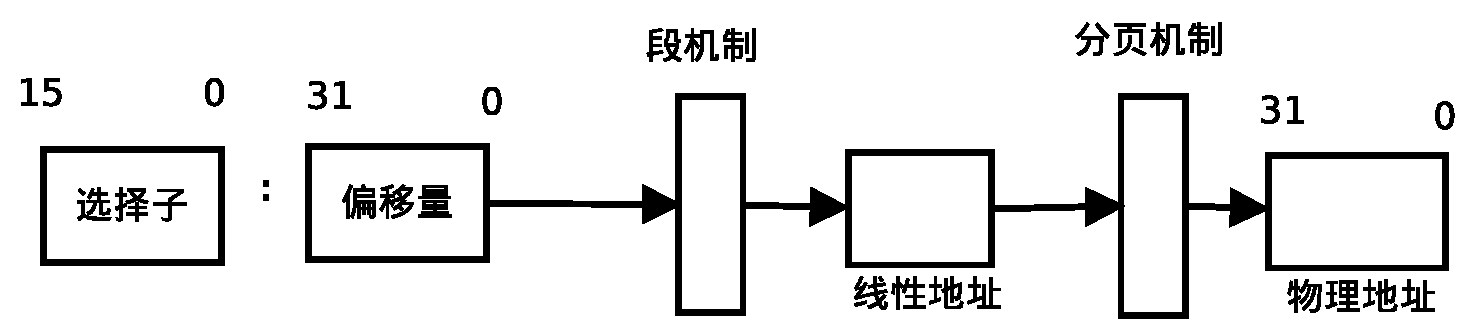
\includegraphics[scale=0.36]{machine.eps}
\caption{地址转换}
\label{machine}
\end{figure}

而在建立起基本段页式管理机制后整个内存看起来像图\ref{neicun}所示:
\begin{figure}[htp]
\centering
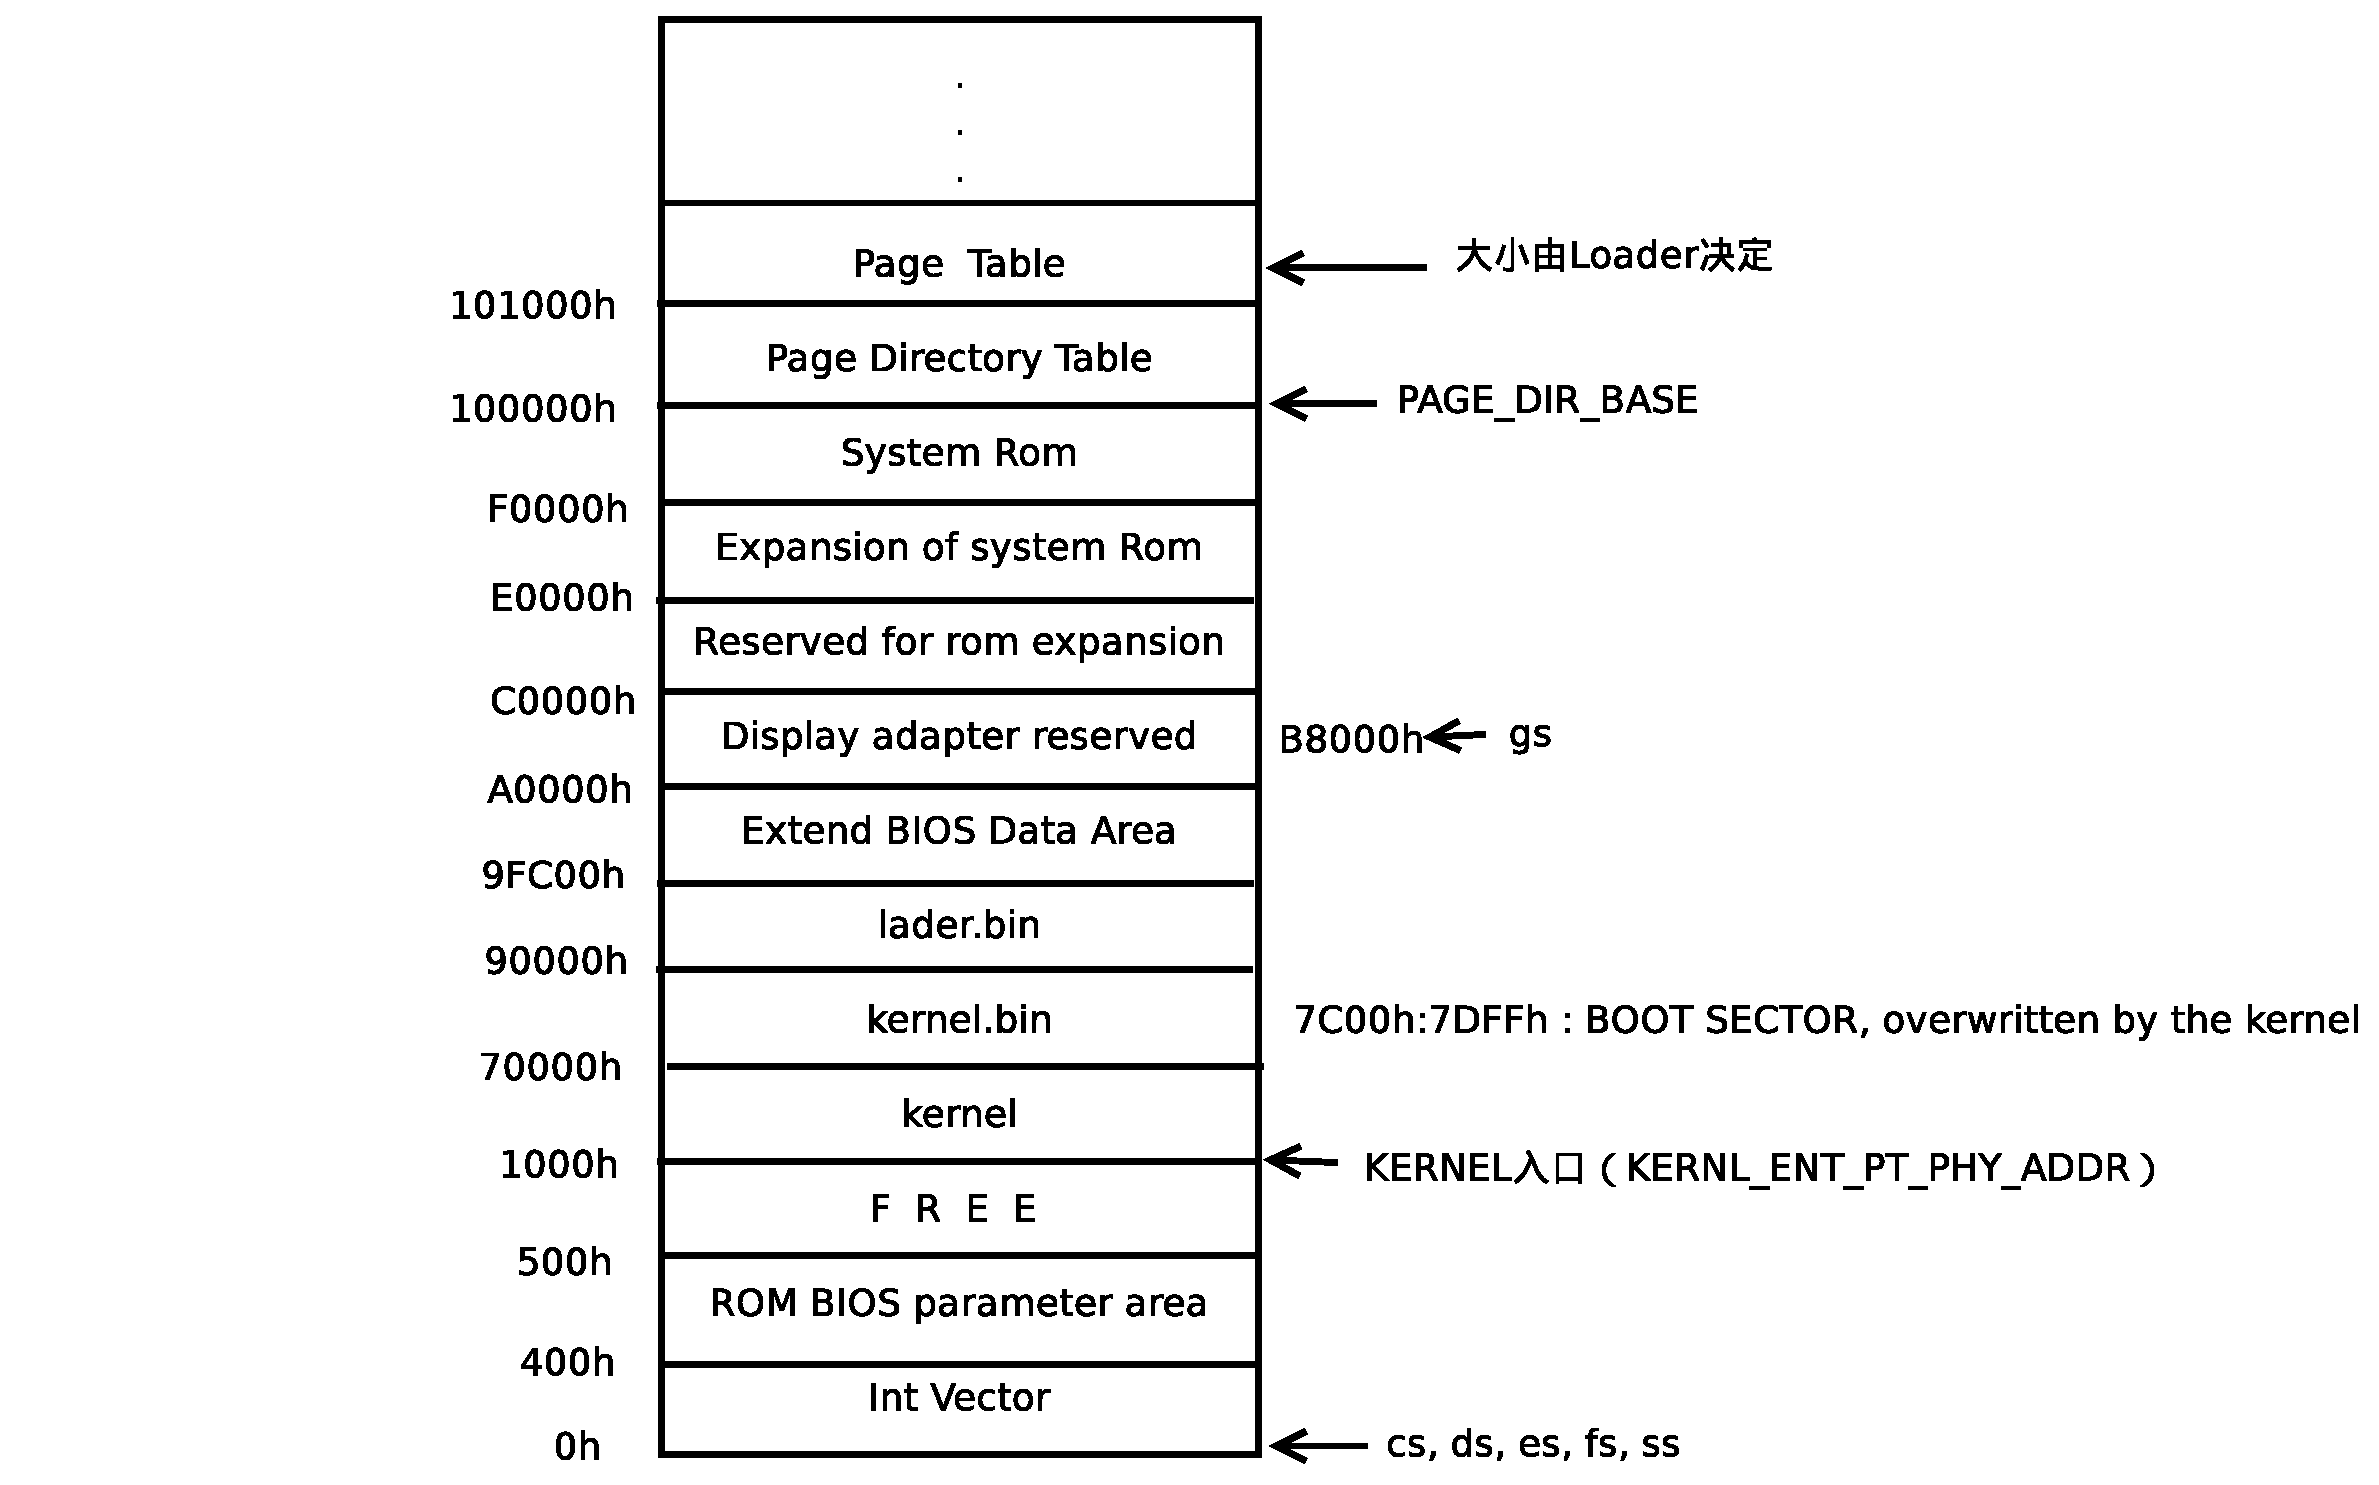
\includegraphics[scale=0.36]{neicun.eps}
\caption{内存概况}
\label{neicun}
\end{figure}

\section{基本分段管理机制}
段是实现虚拟地址到线性地址转换机制的基础。在保护方式下,每个段由如下三个参数进行定义:段基地址(Base Address)、段界限(Limit)和段属性(Attributes)。用于表示上述定义段的三个参数的数据结构称为描述符。每个描述符长8个字节。在保护方式下,每一个段都有一个相应的描述符来描述。按描述符所描述的对象来划分,描述符可分为如下三类:存储段描述符、系统段描述符、门描述符(控制描述符)。在操作系统中定义了三个描述符,分别是一个0~4GB的可执行段、一个0~4GB的可读写段和一个指向显存开始地址的段。
\begin{lstlisting}
;form boot/loader.as
LABEL_GDT:               Descriptor     0,      0,      0
LABEL_DESC_FLAT_C:	Descriptor     0,      0fffffh,DA_CR  | DA_32 | DA_LIMIT_4K
LABEL_DESC_FLAT_RW:	Descriptor     0,      0fffffh,DA_DRW | DA_32 | DA_LIMIT_4K
LABEL_DESC_VIDEO:	Descriptor	 0B8000h,  0ffffh, DA_DRW | DA_DPL3	         
\end{lstlisting}
上面所定义的几个段是在loader中定义的,在内核中本设计使用本设计又将写描述符写入了相应的寄存器。主要是填充了GDT(global Descriptor Table)和LDT(Local Descriptor Table)。

函数cstart()首先把位于Loader中的GDT全部复制给新的GDT,然后吧gdt\_ ptr中的内容换成新的GDT的基地址和界限。这样操作系统中基本的分段管理机制就建立起来了。
\section{基本分页管理机制}
操作系统使用传统的两级也表对物理内存进行管理。使用两级页表一方面是由于x86硬件上支持两级页表,另一方面本设计可以通过减少第二级也表页表项数量来节省内存。本操作系统的两级页表结构如图\ref{page}所示。
\begin{figure}[htp]
\centering
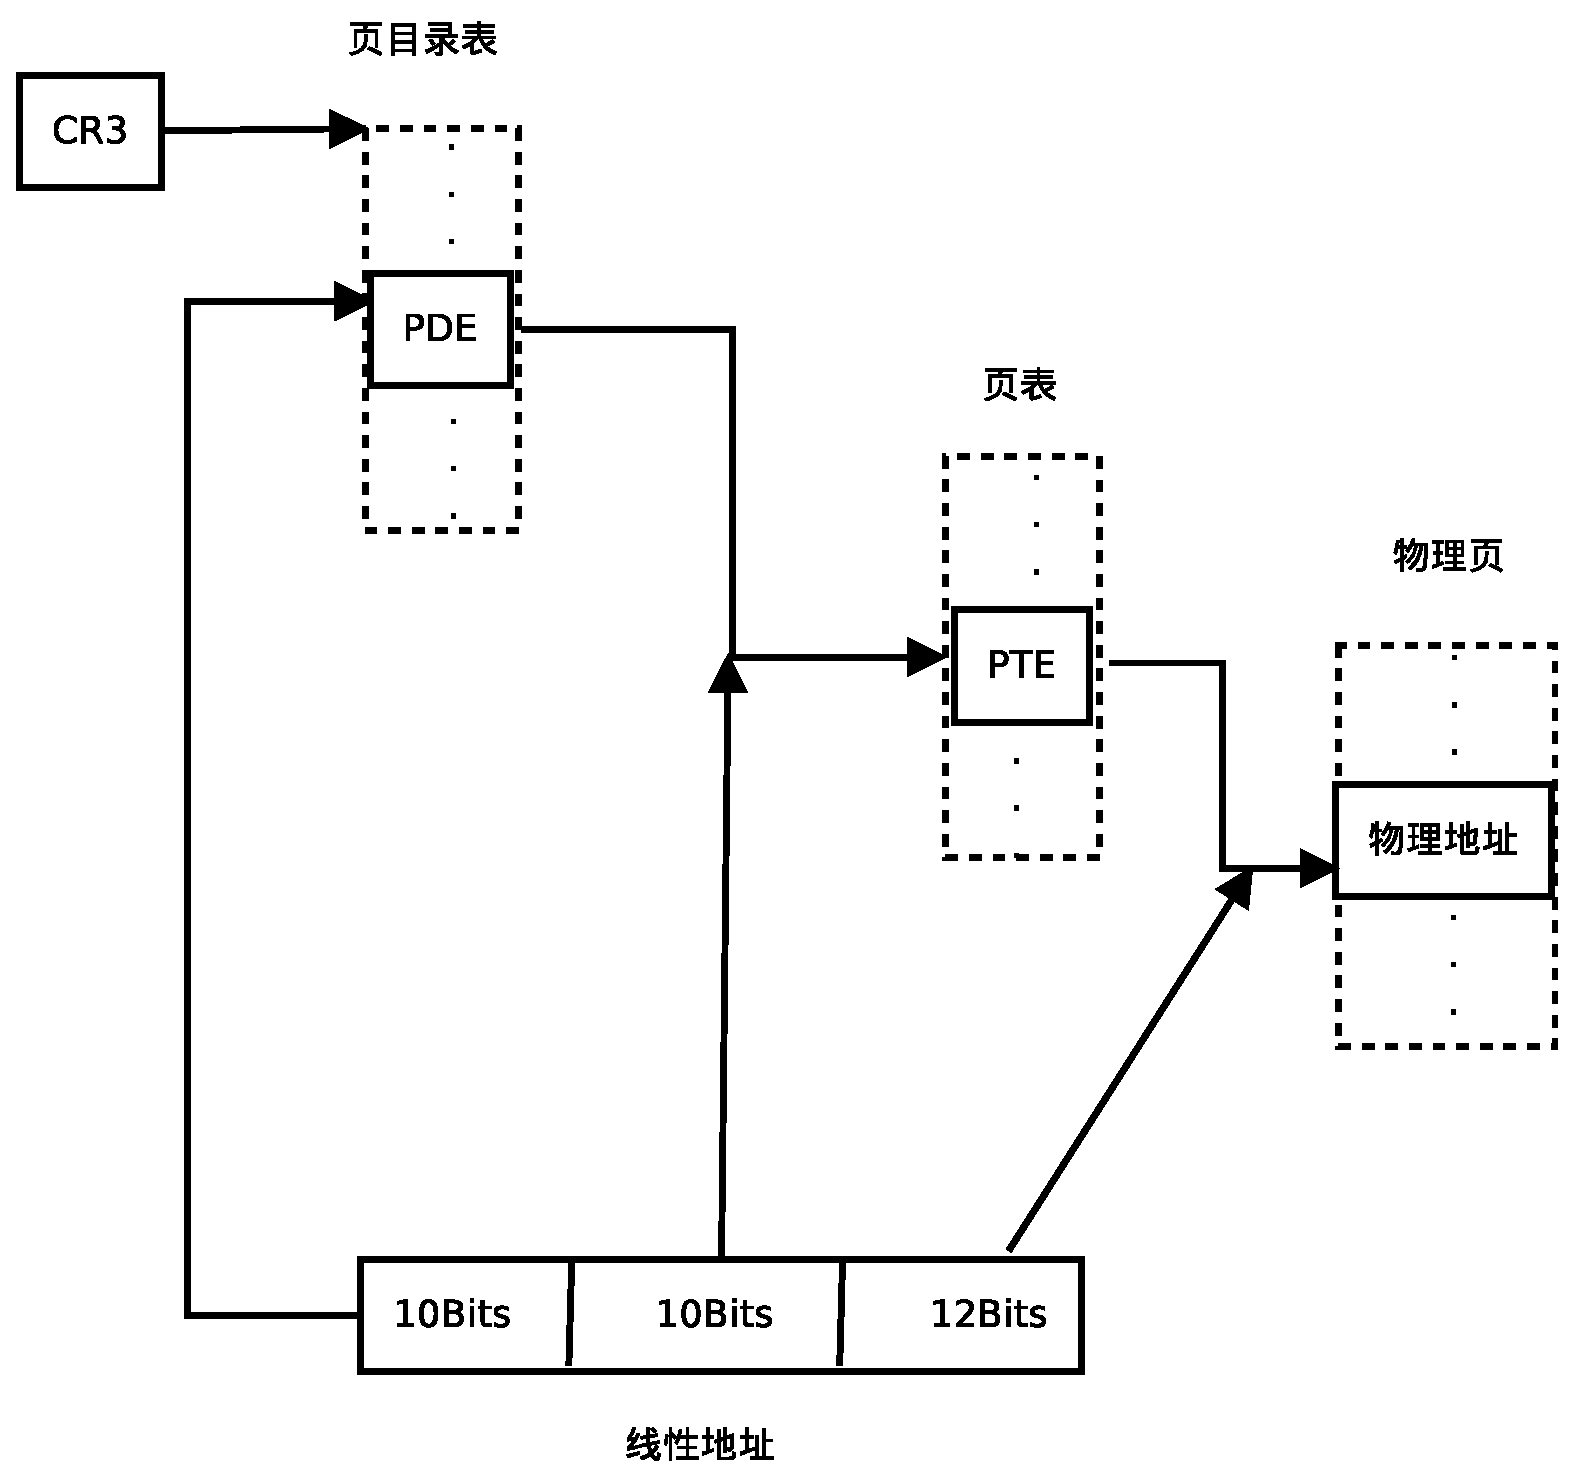
\includegraphics[scale=0.4]{page.eps}
\caption{两级页表}
\label{page}
\end{figure}

\indent \ \ 
第一级也表叫做页目录,大小为4KB,存储在一个物理页中,每个页表项4B,总共有1024个页表项。每个页表项对应着第二级页表的一个页表,第二级页表的每个页表也有1024个表项,每一个表项对应一个物理页。页目录表的表项简称PDE(Page Directory Entry),页表的表项简称PTE(Page Table Entry)。进行转换事,首先是寄存器cr3指定的页目录中根据线性地址的高10位得到页表地址,然后在页表中根据线性地址的第12到21位得到物理页首地址,将这个首地址加上线性地址低12位便得到了物理地址。这里在地址映射的时候采用了直接映射的方法。
基本分页管理机制是在Loader中启动的。
\begin{lstlisting}
;form boot/loader.asm
	call	DispMemInfo ;获取内存情况
	call	SetupPaging ;启动分页机制
\end{lstlisting}
\section{用户内存空间管理}
\indent \ \ 
一个成熟的内存分配机制是比较复杂的,但这并非就意味着简单的机制完成不了这个功能。在这里本设计使用了一种极其简单而且古老的方案,即采用固定分配方式。有新的进程需要内存,就给它划出一定的内存。本设计将大小定为1MB,这个数字在一定程度内可以任意选取,但至少大于内核的大小240KB,这样就能够容的下初始进程Init。然而,并非所有的内存都能够被内存管理程序使用。0~1MB的空间被内核使用,显然不能用。另外未见系统也在内存中开辟出了一些空间充当缓存,这些也不能用。综合各种因素,本设计定义了下面这样几个宏:
\begin{lstlisting}
/*form include/sys/proc.h
 * All forked proc will use memory above PROCS_BASE.
 *
 * @attention make sure PROCS_BASE is higher than any buffers, such as
 *            fsbuf, mmbuf, etc
 * @see global.c
 * @see global.h
 */
#define	PROCS_BASE		0xA00000 /* 10 MB */
#define	PROC_IMAGE_SIZE_DEFAULT	0x100000 /*  1 MB */
#define	PROC_ORIGIN_STACK	0x400    /*  1 KB */
\end{lstlisting}
本设计将PROCS\_ BASE定义为0xA00000,也就是说,将10MB以上的内存空间给用户进程使用。每一个进程占1MB的空间。在进程创建时只需要在用户空间中,拿出1MB给其使用就可以。这样内存分配实现起来就非常方便。这种内存分配方案,其实就是在进程PID和进程内存空间之间建立了一种映像关系,或者说,内存空间基址是进程PID的一个函数。这一方案的缺点非常明显。对于小一点的进程,1MB空间太浪费,而对于大一点的程序,1MB又可能会不够。不过本设计这里偏重于实现。在本设计的操作系统中没有程序大小超过1MB,所有的程序都能够获得足够的内存空间。而对于占用空间很小的程序,这种分配机制存在明显的浪费,但是本设计这里着重于实现,对于这样的优化问题先不予考虑。
\chapter{文件系统}
文件是信息的集合,文件可以是语言程序,目标程序,数据和其他信息。文件一般记录在存储介质如软盘和硬盘上。在本设计所设计的操作系统中,存储文件的介质默认为ATA硬盘。所谓文件系统,就是指操作系统中与文件管理有关的那部分软件和有关文件管理所需要的数据结构的集合,这些数据结构包括文件的各级目录,文件分配表等。从系统的角度来看,文件系统是对文件存储器的存储空间进行组织分配,负责文件的存储并对存入的文件进行保护,检索的系统。具体说,它素则为用户建立、删除、存入、读取、修改、转寸文件,并控制文件的存取。从用户的角度来看,当用户要求系统保存一个已命名的文件时,文件系统根据一定的格式将它的文件存放到文件存储器适当的地方,当用户要使用文件的时候,系统根据用户给出的文件名,能够从文件存储器中找到所需要的文件或文件的某个记录。因此,文件系统的用户,只要知道他们文件的名字,就可以获取文件中的信息,而无需知道这些文件在什么地方和怎样存放。在文件系统的支持下,操作系统才能够方便的使用各种语言编译程序、联机数据、子程序库等。此外所有输入输出操作都能够得到文件系统的服务。
\paragraph{}
\indent \ \ 文件的物理组织设计到文件在文件存储器中的存储方式。文件组织方法取决于用户通常怎样建立这个文件,以后怎样处理,主要的是,也取决与存储介质本身的特征。
\paragraph{}
\indent \ \ 参考一下FAT12文件格式后发现一个简单的文件系统大致需要这么几个要素:要有地方存放Metadata;要有地方记录扇区的使用情况;
要有地方来记录任一文件的信息,比如占用了那些扇区等;
要有地方存放文件的索引。于是根据这些要素,同时参考Minix文件系统,本设计把本设计的文件系统设计成了如图\ref{file}所示。
\begin{figure}[htp]
\centering
\includegraphics[scale=0.4]{file.eps}
\caption{文件物理组织}
\label{file}
\end{figure}
可以看到,总体上来看,它几乎把前述的各个要素实现了:要有地方存放Metadata——占用整整一个扇区的superblock;要有地方记录扇区的使用情况——sector map;要有地方来记录任一文件的信息,比如占用了那些扇区等——inode map以及称作inode\_ array的i-node真正存放地;要有地方存放文件的索引——root数据区。
\paragraph{}
\indent \ \ 
superblock通常也叫超级块,关于文件系统的Metadata本设计都记载这里。sector map是一个位图,它用来映射扇区的使用情况,用1表示扇区已经被使用,0表示未被使用。i-node是UNIX世界各种文件系统的核心数据结构之一,本设计把它借用过来。每个i-node对应一个文件,用于存放文件名、文件属性等内容,inode\_ array这个数组就是把所有i-node都放在这里,形成一个统一的管理机制。而inode map就是用来映射inode\_ array这个数组使用情况的一个位图,用法与sector map类似。root数据区类似于FAT12的根目录区,但本质上它也是一个普通文件,由于它是所有文件的索引,所以本设计把它单独看待。为了简单起见,本设计的文件系统暂不支持文件夹,也就是说用来表示目录的特殊文件只有这么一个。这种不知吃文件夹的文件系统叫做扁平文件系统(Flat File System)。
\chapter{结论与展望}
\section{结论}
经过十二周的时间之后,终于初步完成了我的毕业设计。将一个操作系统的大体框架写了出来。虽然这个操作系统看起来还有很多的地方不进人意,但是已经能够完成操作系统的大部分功能。它有了一套完整的进程管理体系,能够创建和撤销进程,并根据一定的调度算法对并发执行的进程进行调度。同时,还支持多级中断,允许中断嵌套。它有了一套内存管理机制,比较好的管理系统内存资源和用户空间,而且还有一个简单的文件系统,能够让用户进行简单的文件操作。系统内核结构清晰明了,这是因为使用了微内核结构的缘故。当然为了实现微内核结构,还建立了一套进程间通信的机制——同步IPC。与此同时,还有一个信号量机制的雏形。它作为系统资源的管理者,已经能够对一些资源进行简单的管理,比如CPU、键盘、屏幕。作为用户接口,向程序员用户提供了系统编程接口;向一般用户提供了文本终端的交互接口。
\paragraph{}
\indent \ \ 
在实现操作系统的过程中,我阅读了大量的资料和文献。并参考了前人的一些工作成果。对实现一个操作系统所需要的技术,有了一个初步的了解。同时也以论文的形式将这些关键的技术呈现了出来,方便他人。这个操作系统已经具备了一个典型的操作系统所应该具有的功能,因而可以用于操作系统教学中。当作一个操作系统的简单实例来使用。
\section{进一步工作的方向}
虽然操作系统的框架架设起来了。但无论从那个角度来看,这个操作系统还是很粗糙的。因为当时在做的时候,着重于实现,而忽略了优化。所以系统不能够在实际环境中担当一些工作,比如实时控制类的工作。而且系统中各个模块的功能还存在着不小的欠缺。
\paragraph{}
\indent \ \ 
系统没有一个很好设备管理体系。虽说我所设计的信号量机制在经过一定的修改和扩充之后可以完成设备管理的工作。但是这种设备管理也是粗糙而且不精准的。因而,在以后的工作中需要堆设备管理添加相应的代码,实现一套比较完整的设备管理体系。让操作系统能够更好的管理系统设备资源。
\chapter*{致谢}
\addcontentsline{toc}{chapter}{致谢}
光阴荏苒,日月如梭,在青岛理工大学的四年学习时间即将过去。在漫长的人生旅程中,三年时间并不算长,但对我而言,是磨砺青春、挥洒书生意气的三年,也是承受师恩、增长才干、提高学识的三年。我将以一个新青岛理工人的面貌,重新投入到火热的工作和事业中。在此,谨对培育我的母校、教导我的老师、帮助我的同学们致予最诚挚的谢意和敬意。 在此,我特别要感谢我的论文指导老师王晓燕老师。王晓燕老师,她学识渊博,专业精通,对青岛理工大学教育事业怀着深厚的感情;她诲人不倦,与同学们保持着良好的沟通并经常给予科学的指导和热心的勉励。就本篇毕业论文总结报告而言,从提纲、草拟、修改到最后定稿,王老师都给予了一而再、再而三的精心批阅,每个环节都凝结老师努力的付出和辛劳的汗水。毋庸讳言,老师的为人处事将成为我人生的座标和里程碑。我还要感谢给予我很多关心和帮助的同学们,三年学习生活使本设计结下深厚的友谊。俗话说天下没有不散之筵席,在毕业之际,我衷心地同学和朋友们在以后的人生道路上越走越宽广,也深深相信在未来的日子里本设计将一路携手前行,会有很多的碰撞和交流,本设计将始终记得本设计曾在青岛理工大学同窗学习,这将是我克服困难、不断前进的精神动力。
\label{exception}
\begin{thebibliography}{99}
\addcontentsline{toc}{chapter}{参考文献}
\bibitem{orange}Orang's\ 一个操作系统的实现[M].于渊.电子工业出版社.2009年9月.
\bibitem{linux}Linux内核分析及变成[M].倪继利.电子工业出版社,2005.9.
\bibitem{machine}计算机组成与结构[M].王爱英主编.清华大学出版社,2007.7
\bibitem{creference}C:\ A\ Reference Manual[M].Samuel P.Harbison III\ Guy \ L.Steele\ Jr.机械工业出版社,2008.4
\bibitem{asseme}汇编语言程序设计[M].齐志儒\ 高福祥.东北大学出版社,2005.3
\bibitem{1}乔磊,齐骥,龚育昌.一种支持可重构混成系统的操作系统设计与实现[D].中国中国科学技术大学,2009.
\bibitem{2}毛德操,胡希明. Linux内核源代码情景分析[M].杭州:浙江大学出版社,2001
\bibitem{7}C.Wright,C.Cowan,S.Smalley.Linux Security Moudle Framework[C].Ottawa,Canada:Ottawa Linux Symposium.2002
\bibitem{3}陈莉君. 深入分析Linux内核源代码[M].北京:人民邮电出版社,2002
\bibitem{4}孙钟秀,费翔林.操作系统教程[M].北京:高等教育出版社,2003
\bibitem{5}李善平,刘文峰.Linux内核2.4版源代码分析大全[M].北京:机械工业出版社,2002
\bibitem{6}W.L.R.Michael A.Harrison, Jeffery D.Protection in Operating Systems[J].Communication of the ACM.1976.

\bibitem{8}Atlas A,Bestavros A.Design and implementation of statistical rate monotonic scheduling in KURT Linux.In:Proc.of the 20th IEEE Real—Time Systems Symp.Phoenix:IEEE Computer Society[C]Press.1999.
\bibitem{8}Maurice J.Bach.UNIX操作系统设计[M】.机械工业出版社.2004
\end{thebibliography}
\appendix
\chapter{用户编程接口}
\section{printf}
功能:在标准终端tty中显示以指定的格式显示内容。使用方法:printf("[变量格式]",变量....)。
\section{close}
功能:关闭指定文件。使用方法:close(文件指针)。成功返回0。
\section{exec}
功能斯蒂芬斯蒂芬:运行制定的程序。使用方法:exec(const char * path)。
\section{fork}
功能:创建一个子进程,子进程内容为父进程的拷贝,成功返回进程PID。使用方法:fork()。
\section{write}
功能:将信息写入一个文件。使用方法:write(int fd, const void *buf, int count)。
\section{getpid}
功能:返回当前程序的pid。使用方法:getpid()。
\section{open}
功能:打开制定的文件或者创建一个文件,成功返回文件指针,失败返回NULL。使用方法:PUBLIC int open(const char *pathname, int flags)。
\section{read}
功能:读取制定文件的信息。使用方法:read(int fd, void *buf, int count)。
\section{syslog}
功能:通过发送消息到文件系统,将系统日志写入硬盘。使用方法:syslog(const char *fmt, ...)。
\section{ulink}
功能:删除一个文件。使用方法:unlink(const char * pathname)。
\chapter{部分源码}
\section{异常处理函数}
\begin{lstlisting}
/*==================================
                            exception_handler
 *-----------------------------------
 *==================================*/
PUBLIC void exception_handler(int vec_no, int err_code, int eip, int cs, int eflags)
{
	int i;
	int text_color = 0x74; /* 灰底红字 */
	char err_description[][64] = {	"#DE Divide Error",
		"#DB RESERVED",
		"—  NMI Interrupt",
		"#BP Breakpoint",
		"#OF Overflow",
		"#BR BOUND Range Exceeded",
		"#UD Invalid Opcode (Undefined Opcode)",
		"#NM Device Not Available (No Math Coprocessor)",
		"#DF Double Fault",
		"    Coprocessor Segment Overrun (reserved)",
		"#TS Invalid TSS",
		"#NP Segment Not Present",
		"#SS Stack-Segment Fault",
		"#GP General Protection",
		"#PF Page Fault",
		"—  (Intel reserved. Do not use.)",
		"#MF x87 FPU Floating-Point Error (Math Fault)",
		"#AC Alignment Check",
		"#MC Machine Check",
		"#XF SIMD Floating-Point Exception"
		};

	/* 通过打印空格的方式清空屏幕的前五行,并把 disp_pos 清零 */
	disp_pos = 0;
	for(i=0;i<80*5;i++){
		disp_str(" ");
	}
	disp_pos = 0;

	disp_color_str("Exception! --> ", text_color);
	disp_color_str(err_description[vec_no], text_color);
	disp_color_str("\n\n", text_color);
	disp_color_str("EFLAGS:", text_color);
	disp_int(eflags);
	disp_color_str("CS:", text_color);
	disp_int(cs);
	disp_color_str("EIP:", text_color);
	disp_int(eip);

	if(err_code != 0xFFFFFFFF){
		disp_color_str("Error code:", text_color);
		disp_int(err_code);
	}
}
\end{lstlisting}
\section{do\_ fork函数}
\label{dofork}
\begin{lstlisting}
/*********************************************************
 *                                do_fork
 *********************************************************
/**
 * Perform the fork() syscall.
 * 
 * @return  Zero if success, otherwise -1.
 *********************************************************
PUBLIC int do_fork()
{
	/* find a free slot in proc_table */
	struct proc* p = proc_table;
	int i;
	for (i = 0; i < NR_TASKS + NR_PROCS; i++,p++)
		if (p->p_flags == FREE_SLOT)
			break;

	int child_pid = i;
	assert(p == &proc_table[child_pid]);
	assert(child_pid >= NR_TASKS + NR_NATIVE_PROCS);
	if (i == NR_TASKS + NR_PROCS) /* no free slot */
		return -1;
	assert(i < NR_TASKS + NR_PROCS);

	/* duplicate the process table */
	int pid = mm_msg.source;
	u16 child_ldt_sel = p->ldt_sel;
	*p = proc_table[pid];
	p->ldt_sel = child_ldt_sel;
	p->p_parent = pid;
	sprintf(p->name, "%s_%d", proc_table[pid].name, child_pid);

	/* duplicate the process: T, D & S */
	struct descriptor * ppd;

	/* Text segment */
	ppd = &proc_table[pid].ldts[INDEX_LDT_C];
	/* base of T-seg, in bytes */
	int caller_T_base  = reassembly(ppd->base_high, 24,
					ppd->base_mid,  16,
					ppd->base_low);
	/* limit of T-seg, in 1 or 4096 bytes,
	   depending on the G bit of descriptor */
	int caller_T_limit = reassembly(0, 0,
					(ppd->limit_high_attr2 & 0xF), 16,
					ppd->limit_low);
	/* size of T-seg, in bytes */
	int caller_T_size  = ((caller_T_limit + 1) *
			      ((ppd->limit_high_attr2 & (DA_LIMIT_4K >> 8)) ?
			       4096 : 1));

	/* Data & Stack segments */
	ppd = &proc_table[pid].ldts[INDEX_LDT_RW];
	/* base of D&S-seg, in bytes */
	int caller_D_S_base  = reassembly(ppd->base_high, 24,
					  ppd->base_mid,  16,
					  ppd->base_low);
	/* limit of D&S-seg, in 1 or 4096 bytes,
	   depending on the G bit of descriptor */
	int caller_D_S_limit = reassembly((ppd->limit_high_attr2 & 0xF), 16,
					  0, 0,
					  ppd->limit_low);
	/* size of D&S-seg, in bytes */
	int caller_D_S_size  = ((caller_T_limit + 1) *
				((ppd->limit_high_attr2 & (DA_LIMIT_4K >> 8)) ?
				 4096 : 1));

	/* we don't separate T, D & S segments, so we have: */
	assert((caller_T_base  == caller_D_S_base ) &&
	       (caller_T_limit == caller_D_S_limit) &&
	       (caller_T_size  == caller_D_S_size ));

	/* base of child proc, T, D & S segments share the same space,
	   so we allocate memory just once */
	int child_base = alloc_mem(child_pid, caller_T_size);

	/* child is a copy of the parent */
	phys_copy((void*)child_base, (void*)caller_T_base, caller_T_size);

	/* child's LDT */
	init_desc(&p->ldts[INDEX_LDT_C],
		  child_base,
		  (PROC_IMAGE_SIZE_DEFAULT - 1) >> LIMIT_4K_SHIFT,
		  DA_LIMIT_4K | DA_32 | DA_C | PRIVILEGE_USER << 5);
	init_desc(&p->ldts[INDEX_LDT_RW],
		  child_base,
		  (PROC_IMAGE_SIZE_DEFAULT - 1) >> LIMIT_4K_SHIFT,
		  DA_LIMIT_4K | DA_32 | DA_DRW | PRIVILEGE_USER << 5);

	/* tell FS, see fs_fork() */
	MESSAGE msg2fs;
	msg2fs.type = FORK;
	msg2fs.PID = child_pid;
	send_recv(BOTH, TASK_FS, &msg2fs);

	/* child PID will be returned to the parent proc */
	mm_msg.PID = child_pid;

	/* birth of the child */
	MESSAGE m;
	m.type = SYSCALL_RET;
	m.RETVAL = 0;
	m.PID = 0;
	send_recv(SEND, child_pid, &m);

	return 0;
}

\end{lstlisting}

\end{document}
